
\documentclass[12pt,a4paper]{report}
% This document template assumes you will use pdflatex.  If you are using
% latex and dvipdfmx to translate to pdf, insert dvipdfmx into the options.

\usepackage{Bath-CS-Dissertation}
\usepackage{graphicx}
\usepackage{float}  
\graphicspath{ {./images/} }

\title{\bf Travel Itineraries Powered by Recommender and Retrieval Augmented Generation}
\author{Alexander George Nakul Mentzelopoulos}
\date{MSc  in Artificial Intelligence\\ 
                                 % E.g.: Bachelor of Science in Computer Science
                                 %       Master of Science in Data Science
      The University of Bath\\
     2024}

%%%%%%%%%%%%%%%%%%%%%%%%%%%%%%%%%%%%%%%%%%%%%%%%%%%%%%%%%%%%%%%%%%%%%%%%%%%%%%%%
%%%%%%%%%%%%%%%%%%%%%%%%%%%%%%%%%%%%%%%%%%%%%%%%%%%%%%%%%%%%%%%%%%%%%%%%%%%%%%%%
%%%%%%%%%%%%%%%%%%%%%%%%%%%%%%%%%%%%%%%%%%%%%%%%%%%%%%%%%%%%%%%%%%%%%%%%%%%%%%%%
\begin{document}

\hypersetup{pageanchor=false}

% Set this to the language you want to use in your code listings (if any)
\lstset{language=Python,breaklines,breakatwhitespace,basicstyle=\small}

\setcounter{page}{0}
\pagenumbering{roman}

\maketitle
\newpage

% Set this to the number of years consultation prohibition, or 0 if no limit
\consultation{0}
\newpage

\declaration{Travel Itineraries Powered by Recommender and Retrieval Augmented Generation}{Alexander George Nakul Mentzelopoulos}
\newpage

\hypersetup{pageanchor=true}

\abstract
For decades, travel agents have relied on their expertise to curate personalized itineraries for a global clientele. This process has traditionally been manual, with limited automation. This work introduces a novel, fully automated AI-powered travel itinerary generator. The system leverages a review-powered recommender system coupled with the natural language generation capabilities of Large Language Models (LLMs) to learn user preferences and generate unique, personalized itineraries. The proposed approach employs a user preference survey to gather data and build user profiles. These profiles are then utilized for content-based filtering, informing recommendations for the user's itinerary. The recommendations are subsequently fed into an LLM endpoint, which employs a few-shot prompt engineering technique to craft a travel itinerary. Finally, the system retrieves relevant travel component data such as prices and weblinks for presentation to the user.
An initial demonstration of the system in Athens, Greece, highlights its ability to meet user requirements and generates largely positive user feedback. However, a critical evaluation also reveals the potential for "logistical hallucinations" within the generated itineraries. The paper concludes by proposing future directions to address this limitation and explores potential user-requested features for further development.

\newpage

\tableofcontents
\newpage

\listoffigures
\newpage


%%%%%%%%%%%%%%%%%%%%%%%%%%%%%%%%%%%%%%%%%%%%%%%%%%%%%%%%%%%%%%%%%%%%%%%%%%%%%%%%
%%%%%%%%%%%%%%%%%%%%%%%%%%%%%%%%%%%%%%%%%%%%%%%%%%%%%%%%%%%%%%%%%%%%%%%%%%%%%%%%
\chapter*{Acknowledgements}

We would like to acknowledge the support of our volunteer users who lent their time to test and give feedback, and to our advisor Raghubir for his valuable support and advice throughout the development of the project.

\newpage
\setcounter{page}{1}
\pagenumbering{arabic}

%%%%%%%%%%%%%%%%%%%%%%%%%%%%%%%%%%%%%%%%%%%%%%%%%%%%%%%%%%%%%%%%%%%%%%%%%%%%%%%%
%%%%%%%%%%%%%%%%%%%%%%%%%%%%%%%%%%%%%%%%%%%%%%%%%%%%%%%%%%%%%%%%%%%%%%%%%%%%%%%%
\chapter{Introduction}

%%%%%%%%%%%%%%%%%%%%%%%%%%%%%%%%%%%%%%%%%%%%%%%%%%%%%%%%%%%%%%%%%%%%%%%%%%%%%%%%
\section{Introduction and Motivation}

Fueled by globalization, travel has witnessed a meteoric rise as a preferred leisure activity on a global scale. As of Q1 2023, international travel has demonstrably rebounded to 80\% of pre-pandemic levels, indicating a resilient industry poised for continued growth despite pockets of geopolitical instability such as the Russia-Ukraine war and the Israel-Palestine conflict. However, detailed trip planning, particularly for first-time destinations, remains a time-consuming endeavor. 
\begin{figure}[h]
    \centering
    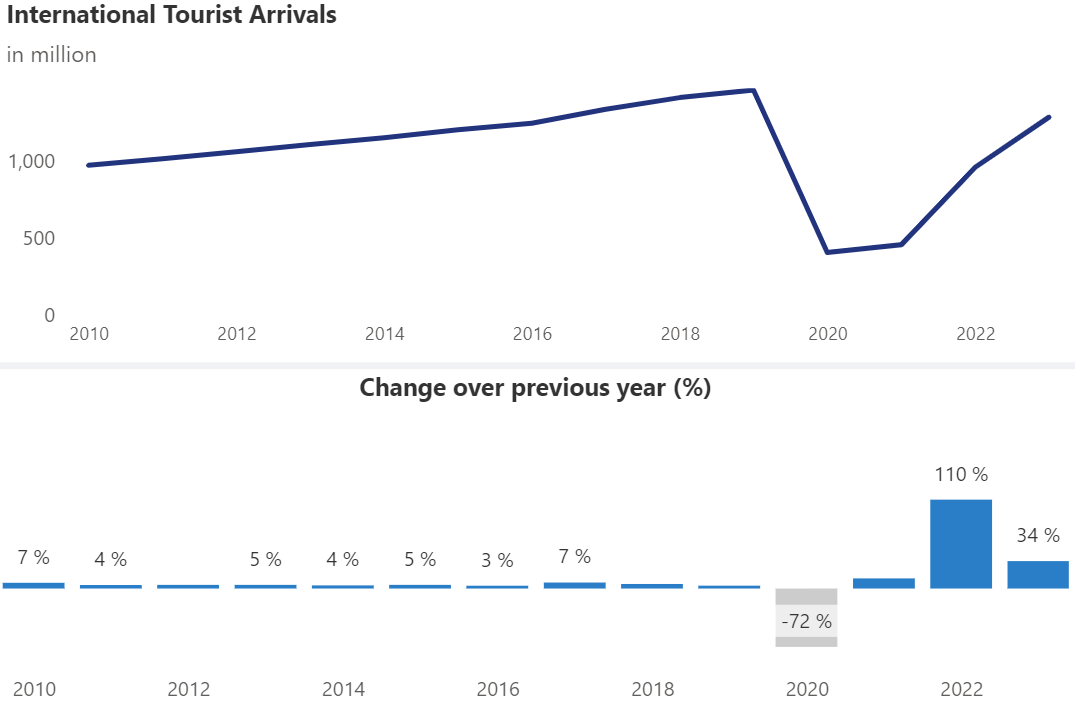
\includegraphics[scale=.5]{tourismgrowth}
    \caption{Tourism Growth Data from UNWTO\citep{unworldtourism}}
\end{figure}

While a plethora of online resources (e.g., TripAdvisor\footnote{TripAdvisor is the largest online travel database that contains information and reviews on travel destinations, restaurants, and attractions}, Booking.com\footnote{Booking.com is one of the largest accommodation booking engines that allow users to search and book hotels at thousands of locations globally}, AirBnB\footnote{AirBnB is one of the largest booking engines to find unique and locally run rental accommodations for travelers worldwide}) empowers comprehensive research, effective itinerary curation necessitates a significant time investment to navigate these platforms and tailor the travel experience to individual preferences and logistical requirements. Traditionally, travel agents served to bridge this gap. However, their services often incur substantial costs and necessitate meticulous communication of travel desires and constraints to facilitate the manual construction of an itinerary. This approach not only proves time-consuming and expensive but also introduces the potential for iterative adjustments and ultimately hinges on the agent's proficiency and knowledge base.


\section{Aims and Objectives}


This paper proposes a novel approach to travel itinerary creation by combining established recommender systems and databases with the text generation capabilities of Large Language Models (LLMs). Our system aims to emulate the personalized service traditionally provided by travel agents, crafting itineraries tailored to individual user preferences and requirements.
Envisioning a paradigm shift from users expending significant time navigating diverse travel blogs and websites, our system strives to collect key user preferences and constraints within a concise timeframe. Subsequently, it will leverage these inputs to generate a feasible travel itinerary that offers a curated selection of personalized options, meticulously culled from the vast repository of travel information available online.
Mirroring the comprehensive service of a travel agent, the proposed itineraries will encompass recommendations for activities, restaurants, and accommodation options, organized into a comprehensive schedule. This itinerary serves as a springboard for user adoption, allowing for customization and personalization to suit individual preferences.
To achieve these overarching goals, a multifaceted system architecture is necessary. Key research questions that must be addressed in this context include:

\begin{enumerate}
\item \textbf{Data Acquisition and Representation:} How can user travel preferences be effectively ingested and stored within the system? What specific data types are necessary, and how can these be optimally sourced?

\item \textbf{Preference-to-Recommendation Mapping:} Given a user's expressed travel preferences, how can the system translate these preferences into a set of well-suited recommendations?

\item \textbf{Itinerary Assembly and Optimization:} Once recommendations are generated for a user, how can these be assembled into a feasible and optimized travel itinerary?
\end{enumerate}


%%%%%%%%%%%%%%%%%%%%%%%%%%%%%%%%%%%%%%%%%%%%%%%%%%%%%%%%%%%%%%%%%%%%%%%%%%%%%%%%
%%%%%%%%%%%%%%%%%%%%%%%%%%%%%%%%%%%%%%%%%%%%%%%%%%%%%%%%%%%%%%%%%%%%%%%%%%%%%%%%
%%%%%%%%%%%%%%%%%%%%%%%%%%%%%%%%%%%%%%%%%%%%%%%%%%%%%%%%%%%%%%%%%%%%%%%%%%%%%%%%
\chapter{Literature and Technology Survey}

\section{The Travel Industry}

\subsection{The Online Travel Agent (OTA) Market}

The online travel agent (OTA) market, encompassing the creation of personalized travel plans for customers, held an estimated value of \$40 billion USD in 2022. This segment is a subset of the broader online travel market, valued at nearly \$500 billion USD\citep{statistatraveldata}. The industry thrives through thousands of companies employing travel agents who curate itineraries for millions of global travelers. Counter to initial predictions of decline due to the internet's rise and platforms like TripAdvisor, coupled with a trend of self-planned trips, especially among younger generations, the OTA market is projected to experience a growth exceeding 6\% annually\citep{linkedinota} .

\subsection{Market Fragmentation and User Demographics}

The user demographics within the OTA industry are multifaceted, leading to a fragmented and diverse market landscape. For instance, adventurous millennials might seek companies specializing in wellness, off-the-beaten-path experiences, or "foodie" adventures, while mature business travelers might prioritize wine tours and business-friendly accommodations.

\subsection{Research Landscape and the Gap in Personalized Itinerary Generation}

While research efforts exist in travel planning (e.g., incorporating points-of-interest based on distance and popularity into tours) \citep{taylortravelitin}, the creation of comprehensive, personalized itineraries using software remains an underexplored territory. Studies like \citet{changlocalitin} in Taiwan have focused on generating strictly local itineraries within a specific origin-destination framework, aiming to streamline self-planned travel, a prevalent mode in that region. Much of the existing research adopts variants of the traveling salesman problem, seeking optimal local routes with the most relevant attractions. Path optimization, undeniably, presents a significant challenge across various domains. However, there is a lack of examples offering personalized travel recommendations beyond traditional travel agencies, let alone software facilitating this discovery process. TripAdvisor, arguably the most recognized repository of travel information, functions primarily as a database, albeit with sorting options based on criteria like ratings and pricing. Given the inherent individuality of travelers, the limited availability of online services capable of automatically generating itineraries tailored to specific preferences is unsurprising. However, the emergence of Large Language Models (LLMs) has witnessed the rise of several services in 2023 that advertise the ability to generate personalized travel information.

\section{The Rise of Large Language Models}

\subsection{LLMs(Large Language Models)}

Large Language Models (LLMs) represent a growing trend within the field of artificial intelligence (AI), particularly in the subdomain of machine learning. These models leverage deep learning algorithms for training, enabling them to interpret, translate, and generate human-like text. LLMs are typically trained on massive datasets of text, often reaching into the billions of parameters. For instance, OpenAI's GPT-3 was trained on a substantial portion of the internet corpus (approximately 1TB of compressed plaintext) and boasts 175 billion parameters\citep{brown2020language}.

While the specific architectural details of many LLMs remain proprietary, the transformer architecture is widely recognized as the foundation for these models\citep{vaswani2023attention}. In essence, LLMs learn the statistical relationships between words within written language. This allows them to predict the next word in a sequence by assigning probabilities to potential continuations.
Consider the following example: "The color of the firetruck is \_." Based on the training data, where "firetruck," "color," and "red" frequently co-occur, the LLM would likely assign the highest probability to the word "red" as the next word in the sequence.

Despite the significant computational resources required for training, LLMs offer remarkable capabilities. They can generate unique and creative text formats based on prompts and instructions provided by users.
The pursuit of the "best" LLM has intensified competition within the AI landscape. Leading companies such as Google, Meta, OpenAI, and Anthropic have actively released various LLM models, with a continuous trend towards larger and more complex architectures. Notably, current research suggests a near-linear correlation between performance and model size (parameter count and compute resources)\citep{aghajanyan2023scaling}. In simpler terms, increasing these factors appears to directly improve LLM performance, with diminishing returns yet to be observed as a significant limiting factor.

\subsection{LLM Performance Benchmarks}

Below in figure 2.1, we can observe the purported performance compared side-by-side of the latest releases of several of these behemoth LLMs.

\begin{figure}[h]
    \centering
    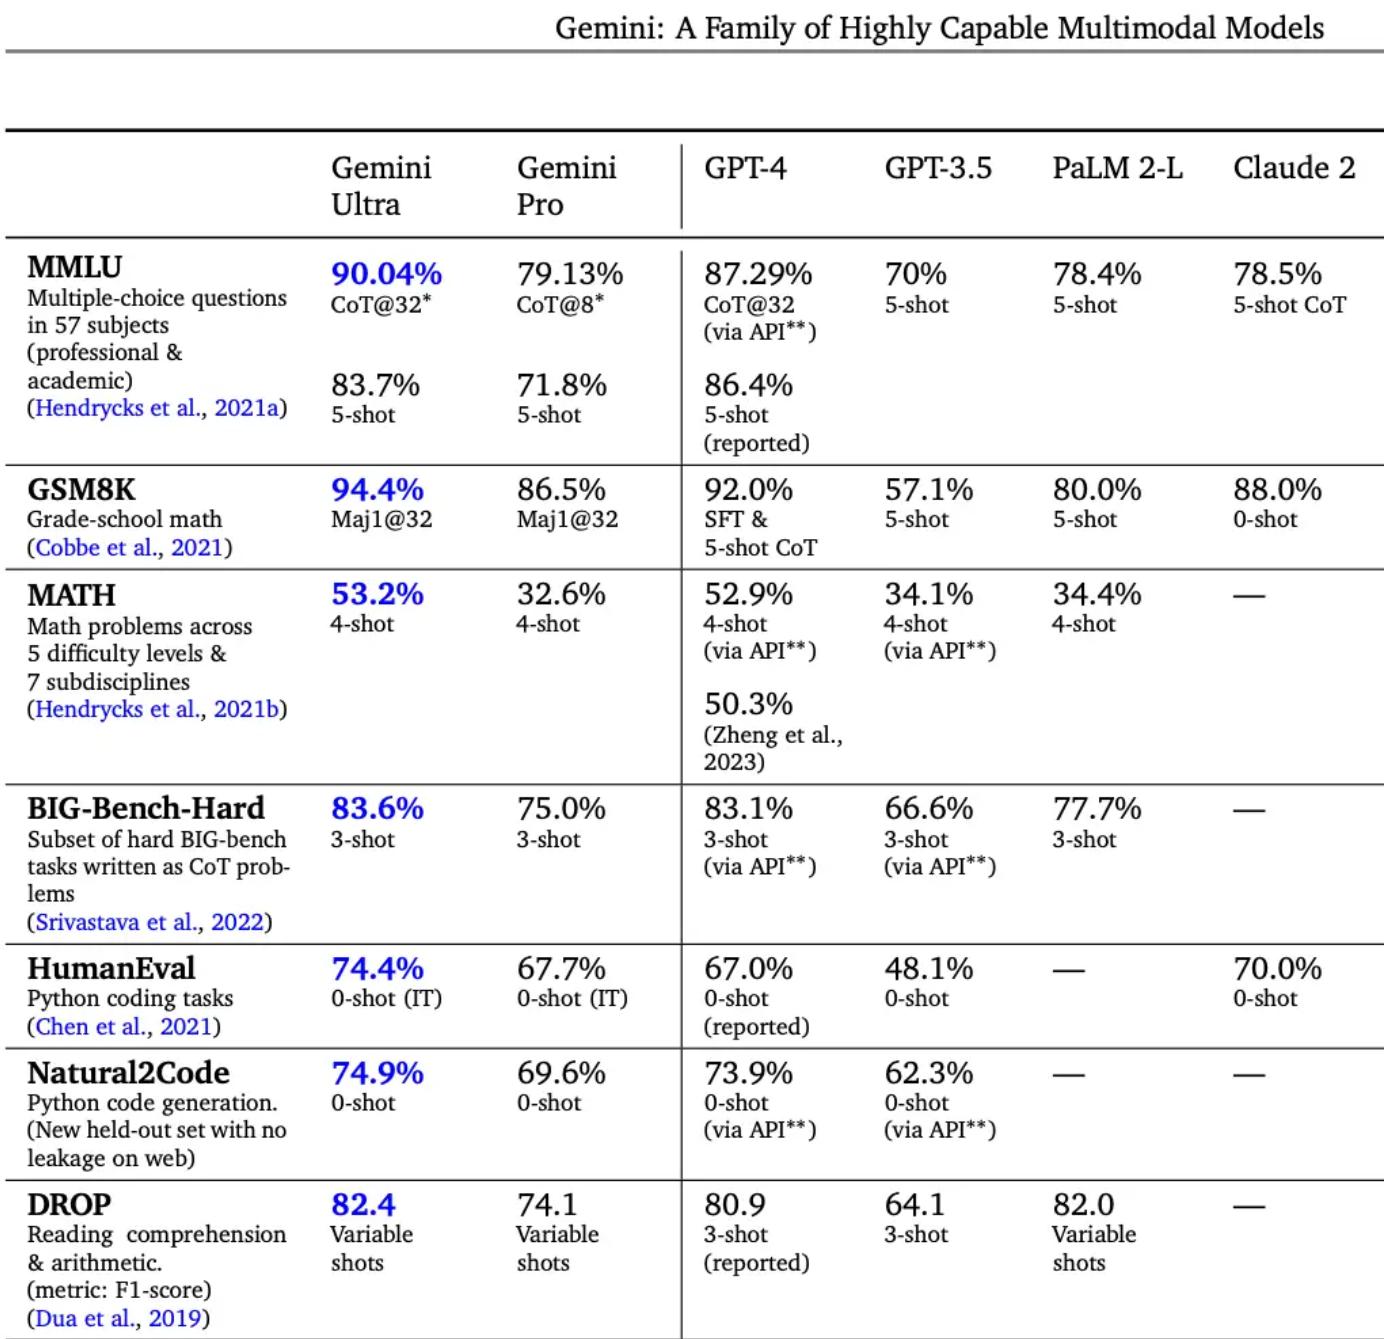
\includegraphics[scale=.8]{llmperformancechart}
    \caption{LLM Performance Benchmarks\citep{geminireport}}
\end{figure}

Evaluating Large Language Models (LLMs) presents a multifaceted challenge.  A significant concern lies in potential data leakage, where an LLM's training data overlaps with the evaluation benchmarks. This leakage can artificially inflate performance metrics, leading to misleading results.

However, in the context of travel information retrieval, the focus of this study is on the practical application of LLMs. While there might be minor idiosyncrasies between different models, their performance on a broad spectrum of tasks, including those relevant to travel, suggests a level of convergence. This convergence allows a degree of confidence in their ability to generate pertinent travel information, despite the acknowledged complexities of LLM evaluation.

\subsection{Hyperparameter Tuning for LLM Text Generation}

Pre-trained LLMs accessible through APIs often provide users with the ability to fine-tune the generation process via a small set of hyperparameters. These hyperparameters significantly influence the characteristics of the generated text, offering a layer of control beyond the initial prompt. Three commonly used hyperparameters for text generation with LLMs include Top-p sampling, Top-k sampling, and temperature.


\subsubsection{Top-p Sampling (Nucleus Sampling)}

Top-p sampling aims to balance the trade-off between diversity and coherence in the generated text. It introduces a probabilistic element while maintaining a focus on high-probability tokens. Here's how it works:

\begin{enumerate}
\item{The model ranks all possible tokens in its vocabulary based on their likelihood (probability) of appearing next in the sequence.}
\item{It then considers only the top-p most probable tokens, where "p" is a user-defined value between 0 and 1. This effectively creates a "nucleus" of high-probability options for selection.}
\item{Within this restricted pool, the model samples the next token based on a probability distribution influenced by the temperature hyperparameter (discussed later).}
\end{enumerate}

Higher values of "p" lead to a wider range of potential tokens being considered, resulting in more diverse and potentially less predictable outputs. Conversely, lower values of "p" restrict the selection to a smaller set of highly probable tokens, yielding more focused and potentially more coherent text. The default value for top-p is typically set to 1.0, allowing the model to consider all tokens in its vocabulary.


\subsubsection{Top-k Sampling} 

Top-k sampling directly controls the number of candidate tokens considered during the selection process. Here's a breakdown:
\begin{enumerate}
\item{The model ranks all tokens in its vocabulary based on their likelihood of appearing next in the sequence.}
\item{It then restricts its selection to the top-k most probable tokens, where "k" is a user-defined integer value.}
\end{enumerate}

A top-k value of 1 essentially forces the model to choose the single most likely token (greedy decoding), potentially leading to repetitive or predictable outputs. Conversely, a higher top-k value, such as 32 (a common default), allows for more exploration within the most probable options, fostering some variation in the generated text. It's important to note that Top-k sampling can be further refined by the Top-p value, as described earlier.


\subsubsection{Temperature}
Temperature acts as a scaling factor, influencing the relative probabilities assigned to candidate tokens during selection. Here's its impact:
\begin{enumerate}

\item{A temperature value greater than 1.0 "softens" the probability distribution, making less probable tokens relatively more attractive to the model. This encourages exploration and can lead to more surprising and diverse outputs, but potentially at the cost of coherence or factual accuracy.}
\item{Conversely, a temperature value lower than 1.0 "sharpens" the probability distribution, further emphasizing the dominance of highly probable tokens. This results in more predictable and focused outputs, potentially lacking creativity but offering greater coherence.}
\end{enumerate}

\section{Model Hallucination}
A significant challenge associated with these models is their susceptibility to "hallucination." Due to their stochastic (probabilistic) nature, LLMs do not possess inherent knowledge or understanding of the information they process. Instead, they rely on statistical patterns learned from vast amounts of training data. This can lead to the generation of novel text that appears plausible but may lack factual grounding. Even when trained on relevant data, LLMs can deviate from accuracy, potentially leading to misleading or nonsensical outputs. These issues highlight the importance of responsible use and critical evaluation of LLM outputs, particularly by non-expert users.

\subsection{Hallucination in Travel Itinerary Generation}
In the context of travel itinerary generation, the most critical risk associated with LLM hallucinations lies in the provision of factually incorrect information. This includes inaccurate details regarding travel destinations, directions, locations, or points of interest. Given the widespread availability of LLMs and their general-purpose nature (trained on massive datasets across various domains), the potential for such errors becomes particularly concerning.



\subsection{Fine Tuning}

Fine-tuning LLMs with domain-specific knowledge and data presents a promising approach to alleviating hallucination in travel itinerary generation. This technique involves enriching the LLM's training corpus with curated datasets encompassing travel guides, tourism information, verified user reviews, and reliable geographical databases. By ingesting such domain-specific content, the LLM can potentially enhance its ability to generate factually accurate and relevant travel itineraries.

There are two primary fine-tuning methodologies: unsupervised and supervised learning. Unsupervised learning involves supplementing the model with raw text data relevant to the travel domain. This can help fill knowledge gaps and refine the LLM's understanding of travel-related concepts. Supervised learning, on the other hand, utilizes a dataset of pre-defined prompts and corresponding responses relevant to travel itinerary generation. By feeding these examples into the model, it learns the desired response patterns to unforeseen prompts within the travel domain. 

Fine-tuning offers the benefit of equipping the LLM with both its original, vast knowledge base and the newly introduced domain-specific expertise. However, it is not without limitations:

\begin{description}
\item{\textbf{Limited Reduction in Hallucination:} While statistically reducing hallucinations, fine-tuning may not entirely eliminate them. Additionally, it remains difficult to determine whether a response is based on the general knowledge or the newly introduced data.}
\item{\textbf{Data Confidentiality Concerns:} Certain information within the travel domain might not be suitable for user access, such as prompts related to other users' travel plans.}
\item{\textbf{Cost and Resource Constraints:} Retraining and maintaining an LLM can be a significant financial burden due to the vast amount of labeled data required for supervised learning.}
\end{description}

\subsection{Few-Shot Learning as an Alternative Approach}

Few-shot learning offers an alternative method for "teaching" LLMs new tasks. This approach involves providing the model with a context prompt (or a series of prompts) that exemplifies how to solve a new problem. Essentially, the model weights remain unchanged, but the prompts serve as explicit demonstrations of how to respond to a specific prompt. Paralleling a form of reinforcement learning, few-shot learning can be a viable method for training LLMs for complex tasks such as travel itinerary generation. Notably, \citet{brown2020language} at OpenAI demonstrated that few-shot prompting can achieve results comparable to those of heavily fine-tuned models.

\section{Retrieval-Augmented Generation}

In addition to fine-tuning and few-shot learning, retrieval-augmented generation presents another promising strategy for controlling LLM outputs and mitigating the risk of hallucination\citep{lewis2021retrievalaugmented}. This approach leverages a comprehensive database alongside the LLM itself. The database is designed for efficient querying using embedding techniques. Here's how it works:

\begin{description}
\item{\textbf{Embedding User Queries:} User queries or prompts are transformed into vector representations (embeddings) that capture their semantic meaning.}
\item{\textbf{Semantic Search:} The LLM's internal database is queried using the user's embedded prompt. This process employs a semantic search engine, allowing for retrieval of the most relevant database entries based on semantic similarity. These entries can be factual information, pre-generated travel elements, or relevant user reviews.}
\item{\textbf{Enhanced LLM Response:} The retrieved information is then used to guide and inform the LLM's response generation process. This can involve incorporating retrieved factual details, leveraging pre-generated travel components as building blocks, or considering user sentiment gleaned from retrieved reviews.}
\end{description}

\begin{figure}[h]
    \centering
    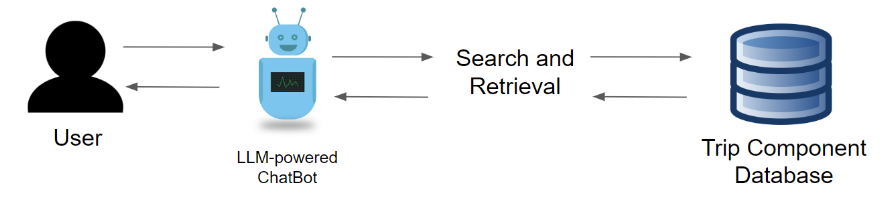
\includegraphics[scale=1.2]{RAGimage}
\end{figure}

Retrieval-augmented generation offers several advantages. Firstly, it allows for maintaining a separate knowledge base, mitigating the need to directly train the LLM on potentially sensitive or vast amounts of information. Secondly, it leverages the strengths of both retrieval systems and LLMs. Retrieval systems excel at efficient factual information retrieval, while LLMs excel at creative text generation. By combining these functionalities, we can potentially enhance the overall accuracy and coherence of the LLM's outputs.

However, there are also considerations to address:

\begin{description}
\item{\textbf{Database Construction and Maintenance:} Creating and maintaining a comprehensive and up-to-date database for the travel domain can be a complex task.}
\item{\textbf{Embedding Technique Selection:} Choosing the optimal embedding technique is crucial for effective semantic search. Different embedding techniques offer varying levels of accuracy and efficiency.}
\end{description}

Retrieval-augmented generation represents a valuable approach for mitigating hallucination in LLM-based travel itinerary generation. By leveraging the complementary strengths of retrieval systems and LLMs, this technique can potentially lead to more accurate, informative, and user-centric travel recommendations.

\section{Travel-specific Chatbots}

The emergence of Large Language Models (LLMs) has demonstrably impacted various domains, including travel. OpenAI's ChatGPT, for instance, offers a glimpse into the potential of LLMs for itinerary generation. However, as shown in the provided Athens itinerary, these outputs often come with disclaimers. The itinerary acknowledges it's just a suggestion and needs user preferences, highlighting the limitations of generic LLM-based approaches.


\begin{figure}[h]
    \centering
    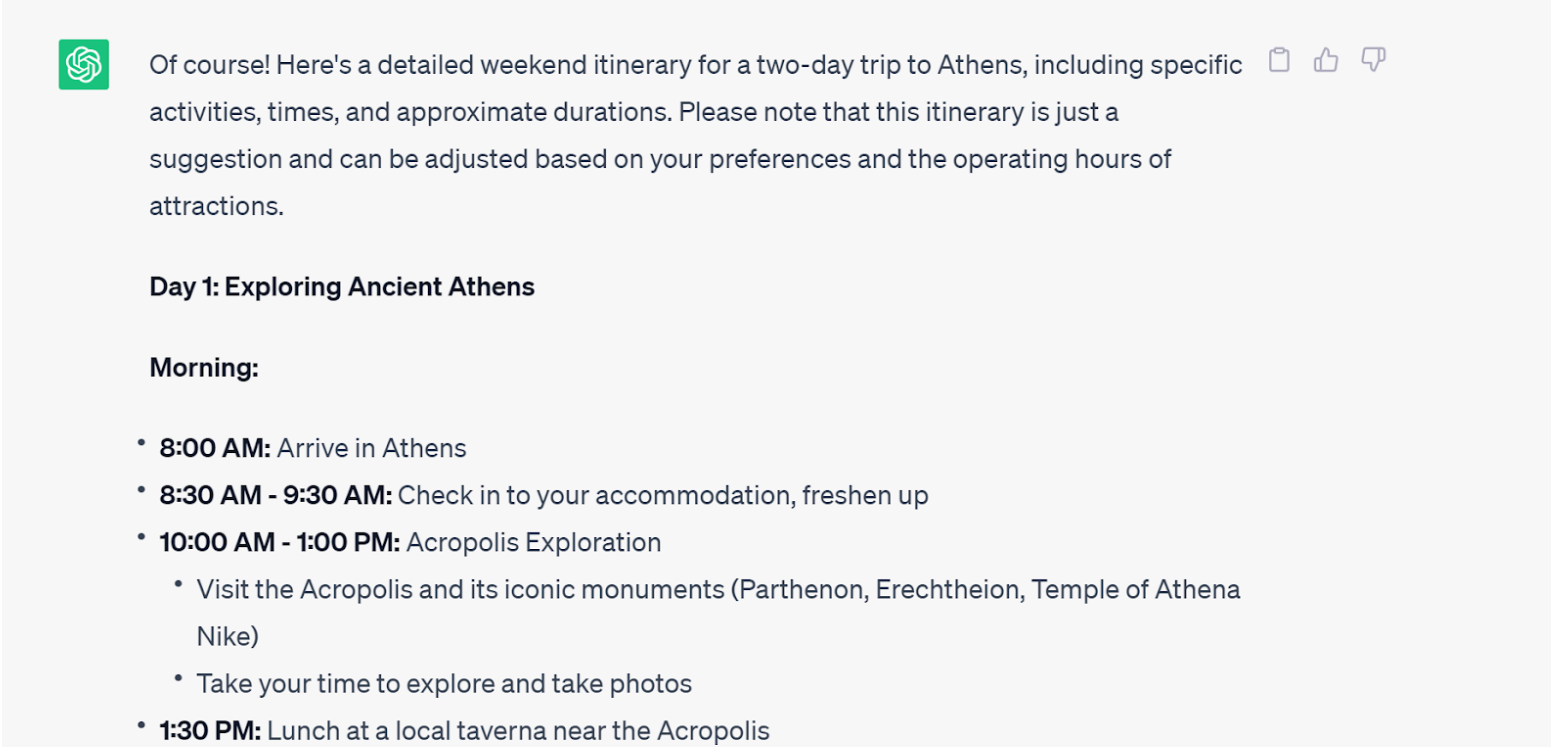
\includegraphics[scale=.75]{chatgptitin}
    \caption{Travel Itinerary Generated by OpenAI's ChatGPT}
\end{figure}


Several companies like MindTrip.ai\footnote{MindTrip was founded in 2023 as a travel agent chatbot that can plan your trip from end to end} have sprung up in response to this gap, promising full trip planning solutions. While these services integrate interesting features like stringing together the whole booking process and flight schedules, the chatbot component often seems like a simple wrapper around existing LLMs. Though some might be fine-tuned to include specific travel info, we were able to prompt the interface to talk about almost anything, like its thoughts on World War II, or if the bot prefers bananas or apples. Additionally, there's no personalization outside of what you tell the agent, which is basically the same as asking one of the LLM providers directly.

In fact, we couldn't find any travel-related model today that could learn a user's preferences and make personalized recommendations. This observation underscores the ongoing quest within the travel industry to leverage AI for truly customized user experiences.



\section{Embedding Techniques}

Given the predominantly textual nature of travel information, efficient search, retrieval, clustering, and other manipulations necessitate embedding this data into vector form. However, short text embedding presents a unique challenge due to sparsity – important words may appear infrequently or only once within a single text snippet. This section provides a brief overview of common embedding techniques.


\subsection{Bag-of-Words (BoW)} A foundational embedding technique frequently used for sentiment analysis, BoW represents text as a collection of constituent words, disregarding word order, grammar, and semantics\citep{mikolov2013efficient}. A vector containing word counts serves as the representation for each text segment (sentence, paragraph, etc.). While BoW offers simplicity, it suffers from high dimensionality caused by sparsity (thousands of words, few appearing in short texts). Additionally, it fails to distinguish synonyms or word order, hindering meaningful clustering of embeddings. As texts lengthen, vector summation tends to converge due to frequent word repetition, limiting its utility for complex manipulations.

\subsection{Term Frequency-Inverse Document Frequency (TF-IDF)} An improvement upon BoW, TF-IDF considers both the frequency of a term within a document (term frequency) and its likelihood of appearing across all documents (inverse document frequency)\citep{grootendorst2022bertopic}. This approach assigns higher weight to terms frequently used within a specific document but rarely encountered across the entire corpus, potentially signifying their significance and information value. However, TF-IDF remains insensitive to word order or semantic similarity.

\subsection{Word2vec} Marking a significant advancement, Word2vec generates embeddings by analyzing the context in which words appear. It employs a neural network to predict the probability of observing context words given a target word, using a sliding window to define the context (e.g., neighboring words before and after the target)\citep{goldberg2014word2vec}. The network's internal parameters are adjusted to optimize these probability predictions. This results in dense, high-dimensional vector representations for each word. Cosine similarity can be used to measure the semantic similarity between words based on these vectors. For instance, "car" and "automobile" will have similar embeddings (high cosine similarity) due to their frequent co-occurrence, while "submarine" and "mountain" will display a lower similarity due to their contrasting contexts.

\subsection{Doc2vec} Building upon Word2vec, Doc2vec introduces a feature vector representing each document\citep{le2014distributed}. Training involves a neural network similar to Word2vec, but additionally updates the document vector, which holds a numerical representation of the entire document. Doc2vec becomes advantageous for classifying longer texts as it can effectively capture their essence through a dense vector useful for sentiment analysis, search, and clustering. As with Word2vec, cosine similarity can be employed to identify or cluster similar documents.

\begin{figure}[H]
    \centering
    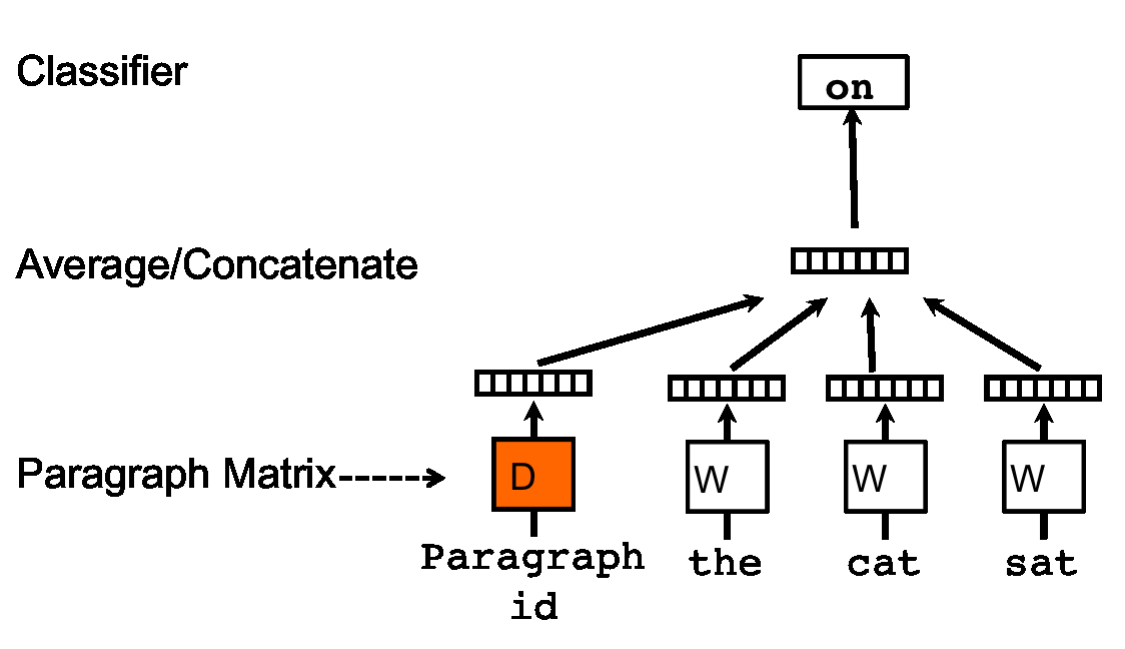
\includegraphics[scale=.6]{doc2vec}
    \caption{Doc2Vec Diagram\citep{le2014distributed}}
\end{figure}

\section{Clustering}

The vast array of clustering algorithms necessitates a selective overview of methods pertinent to travel information and natural language processing. Clustering, inherently an art form within unsupervised learning, often lacks a definitive "true separation" of data.

\subsection{Partitioning-Based Clustering} This family encompasses algorithms like K-means, a centroid-based approach aiming to minimize distances between data points and their assigned cluster centroids\citep{allahyari2017brief}. K-means requires pre-specification of the desired number of clusters and assigns all data points to one. While computationally efficient, its simplicity presents limitations. A significant drawback lies in the necessity of pre-defining the number of clusters, which may not be readily apparent in travel information.

\subsection{Hierarchical Clustering} This family utilizes either agglomerative or divisive strategies. Agglomerative algorithms begin with individual data points and iteratively merge them into larger clusters based on similarity, ultimately represented as a dendrogram\citep{allahyari2017brief}. Divisive algorithms start with all data points in a single cluster and progressively split them based on dissimilarity. Hierarchical clustering can be suitable for text data with an inherent hierarchical structure. For instance, analyzing travel blogs might yield a top-level cluster for "Europe Travel" with subsequent sub-clusters like "Italian Cuisine" and "Hiking in the Alps."

\subsection{Density-Based Clustering} In this family, algorithms like DBSCAN identify clusters based on density\citep{10.5555/3001460.3001507}. Clusters are defined by areas of high density and expand outwards based on the connectivity between a point and its nearest neighbors. Unlike other methods, density-based approaches don't necessarily classify all points into clusters. Some points might be designated as "noise," potentially representing outliers or unique travel destinations within the data. This characteristic can be advantageous for identifying distinct travel experiences that may not neatly fit into pre-defined categories.

\section{Recommender Systems}

Consumer recommender systems generally employ two primary strategies: user-based and item-based filtering.

\subsection{Collaborative Filtering (User-Based)} This approach relies on user profiling and behavior to recommend items to users with similar preferences. Consider Netflix\footnote{Netflix is one of the most popular movie content streaming platforms, well known for their highly successful recommendation engine that provides users with a plethora of content suggestions}, for example. If User A watches "Iron Man," "Star Wars," and "Lord of the Rings," and User B has viewed "Star Wars" and "Iron Man," the system might recommend "Lord of the Rings" due to the users' shared viewing history. The advantage lies in leveraging existing knowledge of user preferences, negating the need to parse item information. However, this requires a pre-existing pool of user data.

\subsection{Content-Based Filtering (Item-Based)} This strategy focuses on the items themselves. Continuing with Netflix, if a user watches several action films, the system might recommend similar films using item metadata like descriptions, genres, actors, directors, etc. The advantage is its ability to function as a "cold start" system, operating without user data. However, it relies heavily on the availability of rich item data and the assumption that recommending similar items is always beneficial. For instance, a user who purchases a guitar for their first lesson on Amazon might not appreciate recommendations for a plethora of other string instruments.

\subsection{Hybrid Approach} The optimal solution often involves a combination of both user-based and item-based filtering, as exemplified by Netflix's successful movie recommendations. Additionally, incorporating other metrics and metadata like popularity can provide valuable suggestions for new users without established user data.

%%%%%%%%%%%%%%%%%%%%%%%%%%%%%%%%%%%%%%
%%%%%%%%%%%%%%%%%%%%%%%%%%%%%%%%%%%%%%%
%%%%%%%%%%%%%%%%%%%%%%%%%%%%%%%%%%%%%%%%%

\chapter{Requirements Analysis and Specification}

\section{User Requirements and Considerations}

Travelers exhibit inherent diversity in their motivations, expectations, preferences, and trip requirements. This project focuses specifically on leisure travelers, excluding those on business trips. To prioritize core functionalities, we have chosen to temporarily defer addressing the user interface (UI) and user experience (UX) design aspects. Our primary focus is refining user input mechanisms and travel itinerary generation capabilities. While the final product is a personalized travel itinerary, acknowledging the need for user input during intermediate steps is crucial for defining their requirements.

A travel itinerary is a comprehensive travel schedule encompassing key elements like accommodations, activities, food, and transportation. Traditionally, travel agents create personalized itineraries by carefully assessing each client's unique needs, preferences, and budget. This typically involves a back-and-forth communication process where the customer relays their requirements (via phone or email) to the travel agent. After iterative discussions exploring preferences and potential concerns, the agent crafts the itinerary.

We aim to replicate this agent-client interaction through a two-phased approach:
\begin{description}
\item{\textbf{Phase I: Requirements and Preference Ingestion}}
\item{\textbf{Phase II: Itinerary Generation}}
\end{description}

\section{Phase I: Requirements and Preference Ingestion}

\subsection{User Experience Considerations:}

\begin{description}
\item{\textbf{Efficiency:} The process of capturing user preferences should be streamlined and time-efficient, particularly when compared to traditional consultations with a human travel agent. Aiming for a completion time under five minutes is a reasonable target.}
\item{\textbf{Data Minimization:} We strive to minimize the amount of requested personal information while ensuring it doesn't compromise the quality of the final itinerary.}
\end{description}

\section{Phase II: Travel Itinerary Output}

The generated travel itinerary must adhere to a set of strict requirements, complemented by additional desirable (but non-essential) features.

\subsection{Content Requirements:}

The itinerary should encompass all essential travel components, including:
\begin{description}
\item{\textbf{Accommodation:} An accommodation option for each night of the trip.}
\item{\textbf{Food:} Restaurant or other food options for breakfast, lunch, and dinner.}
\item{\textbf{Activities:} At least one activity or point of interest for each day.}
\item{\textbf{Transportation:} Information on local transportation options (public transport, taxi, etc.).}
\item{\textbf{Costs:} Approximate costs associated with the aforementioned components.}
\item{\textbf{Feasibility:} All components within the itinerary (restaurants, attractions, accommodations) must be verified to be operational and accessible during the user's travel dates. Additionally, travel logistics and timeframes should be realistic and factual.}
\end{description}

\subsection{User-Preferred Features}

\begin{description}
\item{\textbf{Personalization:} The itinerary content should align with the user's individual preferences, including budget, desired activity types, cuisine choices, and preferred ambiance.}
\item{\textbf{Limited Customization Options:} To enhance user satisfaction, the system should offer a limited degree of control over specific elements within the itinerary, allowing for adjustments if certain aspects don't align with their preferences.}
\end{description}

\section{Critique of Requirements}

While these user requirements establish a solid foundation, there are some aspects that warrant further consideration.

\begin{description}
\item{\textbf{Phase I:} Balancing Efficiency and Comprehensiveness: Achieving a sub-five-minute preference ingestion timeframe might be challenging if the goal is to capture a truly comprehensive understanding of user needs. Travelers often have nuanced preferences or require itinerary flexibility based on unforeseen circumstances. A balance might be struck by offering an initial quick-capture option with the ability to refine preferences later.}

\item{\textbf{Phase II:} The focus on pre-populated activities and restaurants within the itinerary may limit user agency. While pre-populated suggestions are valuable, incorporating user control mechanisms, like allowing users to choose from a curated list or flag preferences for specific activity types (museums vs. historical sites), could enhance user satisfaction.}


\item{\textbf{Addressing the User: Educated Guesses vs. Validated Needs}

It's important to acknowledge that these requirements are currently based on educated guesses about what users might want.  We haven't yet conducted formal user research or testing to validate our assumptions.  To ensure the system caters to actual user needs, incorporating user feedback throughout the development process is crucial.

Conducting user interviews or surveys can help us gather insights into user preferences, travel styles, and pain points.
Usability testing with prototypes can reveal real-world interaction issues and identify areas for improvement in the user input and itinerary presentation. By actively involving users in the process, we can move beyond assumptions and develop a system that delivers a truly personalized and satisfying travel itinerary experience.}
\end{description}



%%%%%%%%%%%%%%%%%%%%%%%%%%%%%%%%%%%%%%%%%%%%%%%%%%%%%%%%%%%%%%%%%%%%%%%%%%%%%%%%
%%%%%%%%%%%%%%%%%%%%%%%%%%%%%%%%%%%%%%%%%%%%%%%%%%%%%%%%%%%%%%%%%%%%%%%%%%%%%%%%
\chapter{Design}

\section{User Preference Ingestion and Data Acquisition}

Building upon the established user requirements, this section proposes a system design to address travel preference ingestion and data acquisition.

\subsection{Travel Preference Ingestion}

The system must capture user preferences efficiently (under 5 minutes) while minimizing the amount of personal information requested.  First, we define "travel preferences" as user inclinations towards specific travel components. Similar to user ratings on platforms like Netflix, these preferences indicate whether a user likes or dislikes a particular activity (e.g., historical museums, walking tours) or accommodation type (e.g., beach resorts).  Unlike Netflix movies, however, travel preferences encompass broader categories: accommodation, food, and activities. These core components are interdependent – accommodation location influences accessible activities, and preferred activities impact dining options.

\subsection{Travel Data Landscape}

The past 15 years have witnessed a significant growth in travel-related data. Platforms like TripAdvisor, Viator, Booking.com, and Airbnb categorize, classify, and allow user reviews for these core travel components.  Travelers have transitioned from relying on guidebooks and tourism companies to independently browsing online resources like TripAdvisor for information and reviews.  Many hotels, restaurants, and attractions also maintain websites with detailed information.

In essence, these companies have created online, searchable databases of travel information, often accessible via APIs. Unlike movie databases with attributes like genre, director, and release date, travel data encompasses entities like restaurants (cuisine, menu, description) and hotels (price, location, description).  The specific data structure varies based on how each company organizes its information.

For this project, TripAdvisor was chosen as the primary data source due to its focus on leisure travel, comprehensive coverage of all core travel components (accommodation, activities, food), and rich metadata (descriptions, cuisine types, and reviews).

\section{Overall Design and Data Acquisition Strategy}

Given a hypothetical database encompassing a vast array of accommodation, activity, and food options, the challenge lies in efficiently determining user preferences while adhering to the time and privacy constraints.  Furthermore, this information should be valuable for predicting future itinerary recommendations.

Several approaches were considered:

\begin{enumerate}
\item{\textbf{Exhaustive User Selection:} Present users with a vast selection of travel components across thousands of possibilities.
\begin{description}
\item{Advantages: Thorough and data-independent}
\item{Disadvantages: Time-consuming (violates 5-minute limit)}
\end{description}}
\item{\textbf{Personal Data Integration:} Utilize additional user data like age, gender, address, social media content, past travel data, or location history to draw correlations between user preferences and personal data.
\begin{description}
\item{Advantages: Potential for more personalized recommendations, potentially quick for user.}
\item{Disadvantages: Privacy concerns, difficulty establishing accurate correlations initially.}
\end{description}}
\item{\textbf{Targeted User Ratings:} Prompt users to rate a limited number of travel components to inform preference prediction for future itinerary components.
\begin{description}
\item{Advantages: Potentially quicker than 5 minutes, data-independent.}
\item{Disadvantages: Careful selection and design of surveyed components are crucial for accurate prediction.}
\end{description}}
\end{enumerate}

While a hybrid model incorporating options (2) and (3) might theoretically offer the most accurate predictions, project limitations and a focus on privacy protection led to the selection of option (3).  Users will be presented with a small set of travel components to rate (yes/no), and this information will be used to infer their preferences and predict suitable components for their personalized travel itinerary.


\section{Building a Travel Component Survey}

Having established the user preference ingestion method, the next crucial step involves selecting a representative subset of travel components for user evaluation. This subset should effectively predict the user's broader preferences within a limited timeframe.

\begin{figure}[H]
    \centering
    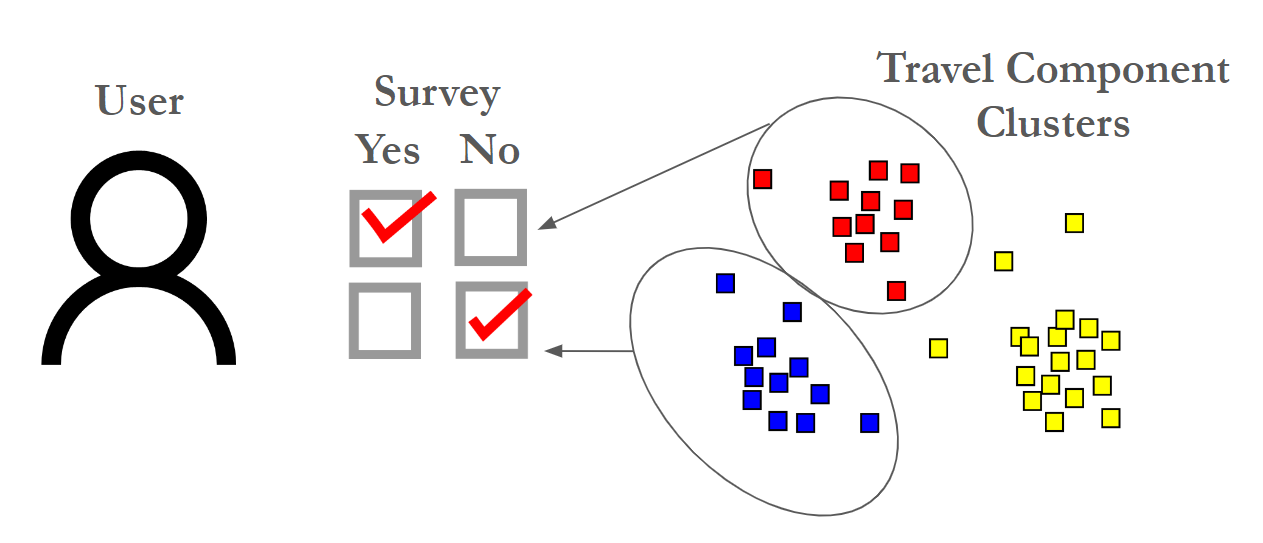
\includegraphics[scale=.6]{travelclusterdemo}
    \caption{Travel Component Clusters to Survey}
\end{figure}

\subsection{Challenges Compared to Movie Recommendations}
Compared to recommender systems like Netflix, selecting representative travel components presents a greater challenge. Movie datasets are more uniform, consisting solely of films with easily identifiable and discrete attributes like genre, director, and actors. Netflix can readily assess user preferences by observing their viewing history of similar films. Additionally, with a large user base and historical data, user-based recommendations become feasible by matching users with similar viewing patterns.

For travel recommendations, the selection process requires additional considerations.  First, location plays a vital role.  Travelers are generally more interested in experiencing local activities and cuisines. While personal preferences exist (e.g., enjoying Chinese food), a user visiting Athens, Greece, likely wouldn't prioritize finding a Chinese restaurant.  Exceptions exist, but user preferences established in familiar locations might not readily translate to foreign destinations.

\subsection{Category-Based Selection Using TripAdvisor Data}
We hypothesize that TripAdvisor metadata (cuisine, description, ratings) can be leveraged to categorize travel components within a specific location.  This categorization can be achieved through data analysis of existing labels or by employing clustering techniques.  Once a categorized dataset is established for the chosen location, a representative component can be selected from each category to serve as the sample set for user evaluation.  By understanding the "kinds" of activities and restaurants a user favors within these categories, the system can recommend similar items across preferred categories.
Provided the number of categories remains manageable and allows for user evaluation within the 5-minute timeframe, this approach should offer good coverage of various travel components while effectively predicting user suitability.

\begin{figure}[H]
    \centering
    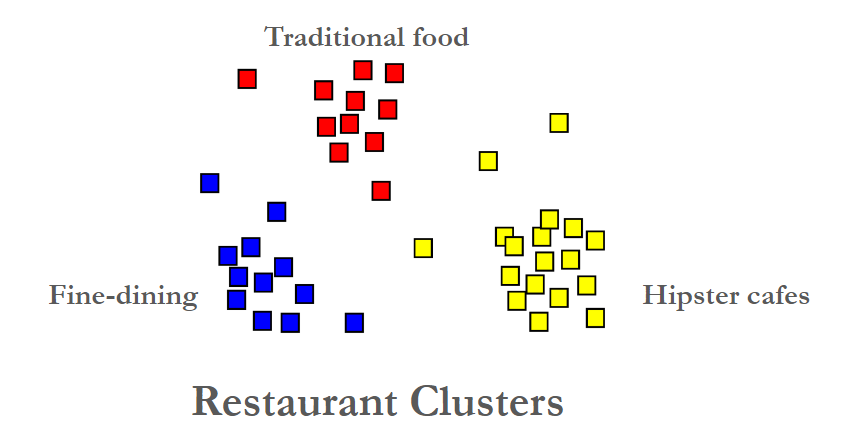
\includegraphics[scale=.8]{exrestaurantclusters}
    \caption{Example Restaurant Clusters}
\end{figure}

\section{Itinerary Assembly: Selecting and Organizing Travel Components}

Building upon the user preference ingestion, this section explores strategies for assembling a personalized travel itinerary.  Traditionally, a travel agent curates itineraries by meticulously selecting components that optimize travel time and prioritize "must-see" experiences.  In the absence of human intervention, we consider alternative approaches:
\begin{enumerate}
\item{\textbf{Rules-Based Algorithm:} This approach involves constructing an algorithm that assembles travel components based on pre-defined rules, leveraging component metadata like geographic location and TripAdvisor ratings.
\begin{description}
\item{Advantages: Offers granular control and customization over itinerary parameters.}
\item{Disadvantages: High complexity due to logistical considerations, component interactions, and potential limitations in scalability across diverse locations.}
\end{description}}

\item{\textbf{Manual Itinerary Templates: }This method involves creating pre-defined itinerary templates with the flexibility to substitute specific components based on user preferences, facilitated by a rule-based program.
\begin{description}
\item{Advantages: Offers greater scalability compared to a purely rules-based approach, as templates can be adapted for different user profiles. Human-crafted templates can also mitigate logistical issues.}
\item{Disadvantages: Requires development of multiple templates potentially for each location, increasing manual workload and scalability challenges.}
\end{description}}

\item{\textbf{Large Language Model (LLM) Integration:} A statistically-driven approach leverages an LLM to generate a plausible travel itinerary from a curated list of travel components.  Prompt engineering plays a crucial role in influencing the model's output.
\begin{description}
\item{Advantages: Generates human-readable formatted itineraries in a scalable and automated manner, minimizing human intervention.}
\item{Disadvantages: Requires careful crafting and fine-tuning of prompts to ensure consistent results. Logistical issues might arise due to potential model hallucinations (generating inaccurate elements).}
\end{description}}
\end{enumerate}
Given the project's focus on reduced complexity and potential future user interaction within the  experience, we opted for the LLM-based approach (option 3).  This entails developing prompts that integrate user travel component preferences to directly generate personalized itineraries.
To maintain project focus as a proof-of-concept, \textbf{Athens, Greece}, was selected as the user's intended travel destination.  This choice is based on its popularity as a tourist destination and our familiarity with the location, which facilitates troubleshooting of generated itineraries.

\begin{figure}[H]
    \centering
    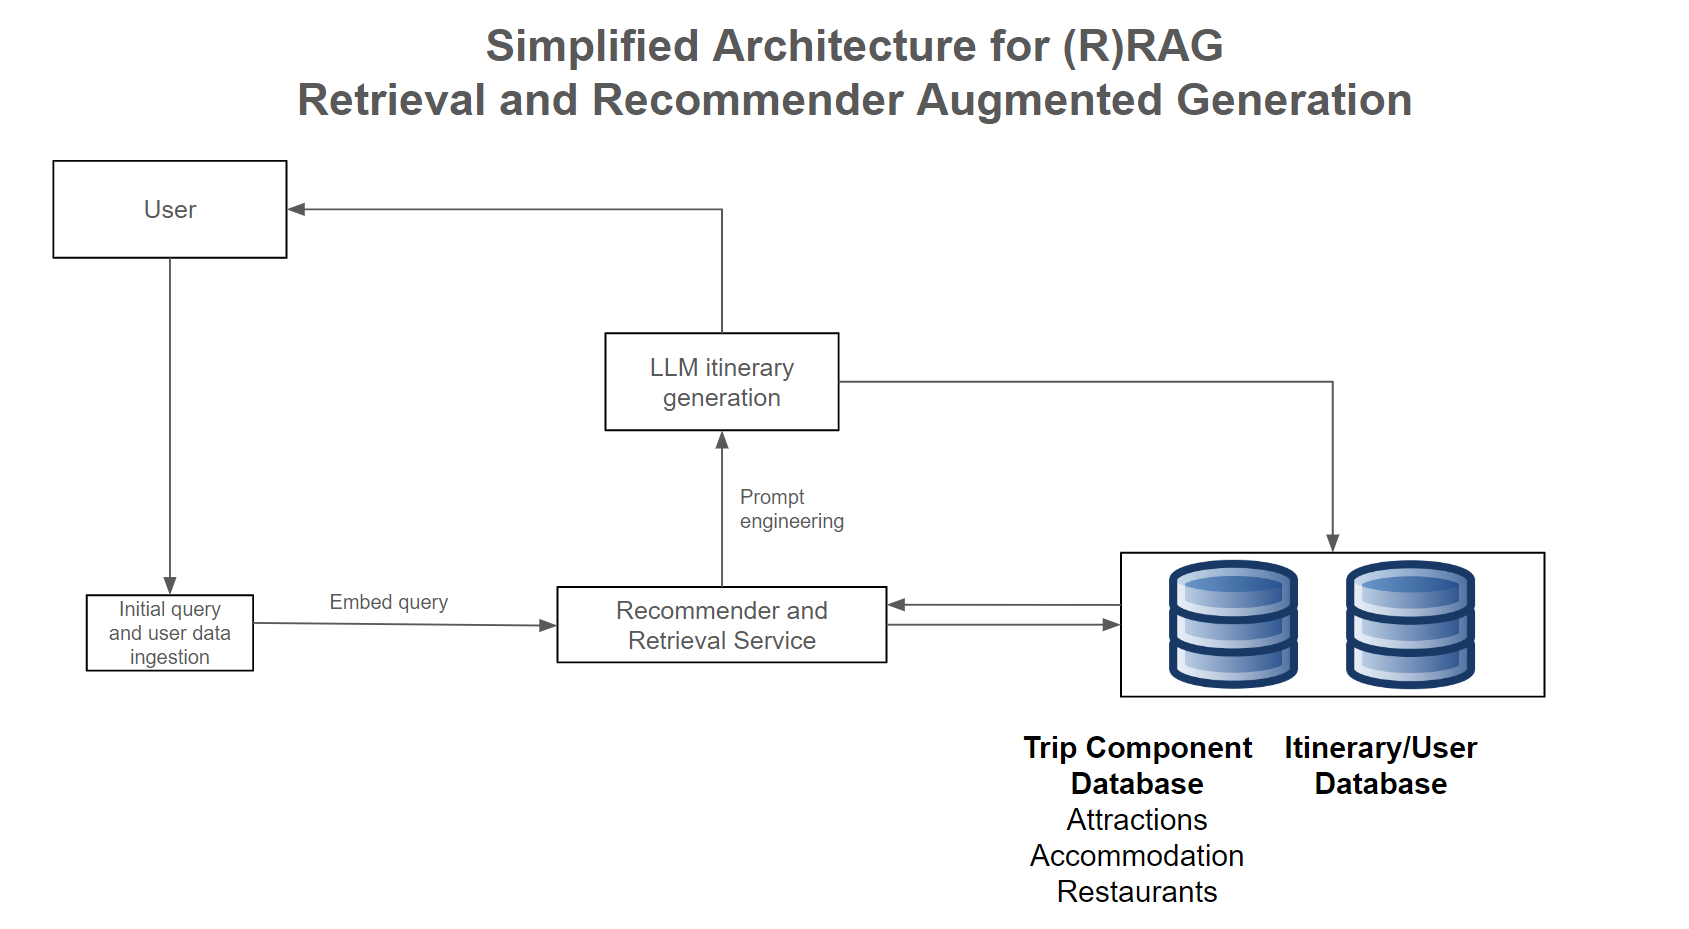
\includegraphics[scale=.7]{systemdiagram}
    \caption{Travel Itinerary Recommender and Generator System Diagram} 
\end{figure}



%%%%%%%%%%%%%%%%%%%%%%%%%%%%%%%%%%%%%%%%%%%%%%%%%%%%%%%%%%%%%%%%%%%%%%%%%%%%%%%%
%%%%%%%%%%%%%%%%%%%%%%%%%%%%%%%%%%%%%%%%%%%%%%%%%%%%%%%%%%%%%%%%%%%%%%%%%%%%%%%%
\chapter{Technical Implementation and Methodology}

\section{Data Acquisition and Preprocessing}

The initial stage involved acquiring raw TripAdvisor data for entities classified under "Athens, Greece." TripAdvisor categorizes entities as restaurants, attractions, or accommodations, a structure we adopted. Each listing comprised over 700 data points.

For brevity, the process of data reduction is omitted here.  This process focused on identifying and retaining relevant columns with accurate data suitable for clustering travel components.

Leveraging the inherent distinctions between these components within a travel itinerary, we opted to divide the data into three separate datasets: hotels, attractions, and restaurants.  These categories possess readily identifiable characteristics and unique metadata (e.g., restaurant menus and cuisines, hotel amenities).

Following data preprocessing and removal of unsuitable entities (low-rated or lacking data), we obtained a refined dataset containing approximately 500 restaurants, 200 hotels, and 300 attractions.

\subsection{Clustering Strategy and Goals}

Our primary objective for data clustering was to achieve the following:

\begin{description}
\item{\textbf{Meaningful Clusters:} Each cluster should exhibit a readily interpretable characteristic, allowing for human comprehension. For example, a cluster might represent "cheap vegetarian restaurants."}
\item{\textbf{Manageable Number of Clusters:} The total number of clusters should remain sufficiently small to facilitate the selection of a representative element from each cluster for the initial user preference survey (ideally no more than 40 clusters across all travel component types).}
\item{\textbf{Distinct Cluster Separation:} Despite the limited number of clusters, they should exhibit clear differentiation in characteristics. For instance, Indian and Chinese restaurants should not be grouped solely based on their shared classification as "Asian cuisine," as a preference for one may not necessarily imply a preference for the other.}
\end{description}

\section{Clustering with Travel Component Metadata}
Our initial clustering approach leveraged various metadata fields for restaurants in Athens, Greece.  These fields included descriptions, approximate cost, cuisine type, and TripAdvisor ratings.  We restricted the dataset to well-rated establishments (above 4.0 stars on TripAdvisor) under the assumption that tourists prioritize highly-rated locations.  This filtering resulted in approximately 500 restaurants.

The data encompassed three primary categories:
\begin{enumerate}
\item{\textbf{Discrete Data:} Categorical variables like cuisine type, which could be readily transformed.}
\item{\textbf{Continuous Data:} Numerical data like TripAdvisor ratings.}
\item{\textbf{Text Data:} Textual information including descriptions, frequently occurring review words, and addresses.
To handle text-based features, we employed a variety of embedding techniques discussed in the literature review(Word2Vec, BagofWords etc).}
\end{enumerate}
We experimented with various clustering algorithms (centroid-based, density-based, distribution-based, and hierarchical) using different combinations of data columns, including the entire dataset. Unfortunately, the resulting clusters exhibited unclear separation, appearing random to human evaluation for certain data subsets.  We attribute this to the following factors:
\begin{description}
\item{\textbf{Limited Categorical Data Diversity:} Splitting clusters based on discrete variables proved challenging due to insufficient data diversity. For example, a significant portion of Athenian restaurants belong to the "Greek" category with "Greek cuisine," limiting the effectiveness of using pre-defined categories or combinations for clustering.}
\item{\textbf{Ineffectiveness of Description Text:} We attempted to leverage restaurant descriptions, which typically comprised 1-3 sentences. Surprisingly, this approach yielded limited success. Many establishments (likely the authors of their own descriptions) employed similar language to express identical sentiments or provided minimal descriptive content.}
Here are some illustrative restaurant description examples:
\begin{description}
\item{\textit{"Atitamos restaurant, in the center of Athens, maintains all the favorite Greek traditional dishes which have been enriched with more interesting tastes. All the dishes are prepared exclusively with fresh and seasonal ingredients. Popular specialties include meat dishes, seafood, fresh fish, a wide variety of mouthwatering appetizers and delicious desserts."}}

\item{\textit{"Welcome to Thinalos Restaurant! Discover the world of wonderful and exquisite seafood dishes we offer, made with fresh ingredients."}}
\end{description}
\end{description}
As you might ponder, perhaps this reflects the inherent similarity between these establishments. While this may hold true for certain segments, our initial hypothesis was that distinct categories existed (e.g., a late-night bar serving small traditional dishes versus a family-friendly Asian restaurant).  Unfortunately, employing metadata alone proved insufficient to achieve clear cluster separation due to the overall lack of data richness and the presence of noise.
Furthermore, user location selection likely extends beyond a simple consideration of ratings and a few keywords.  \textit{Reviews} themselves are likely a more valuable source of user decision-making criteria and could be the crucial key to meeting our cluster criteria above.


\section{Shifting Focus to Review-Based Clustering}

Our initial clustering approach based on metadata yielded limited success.  We propose a new hypothesis:  the content of user reviews for a location possesses a unique "signature."  Furthermore, we posit that the language used to describe similar locations exhibits a degree of similarity, facilitating the grouping of these locations within clusters and the differentiation between distinct clusters.  Essentially, user reviews can be viewed as a more realistic and human-generated form of location description compared to conventional metadata.

The vast majority of locations possess hundreds of reviews, varying in length and quality.  For this clustering approach, we restrict our data to the most recent 50 reviews for each location.  This selection is justified by the following reasoning:
\begin{enumerate}
\item{\textbf{Review Timeliness:} The most recent reviews provide the most up-to-date information regarding a location.}
\item{\textbf{Greater Textual Content:} Fifty reviews, even assuming a few sentences each, offer a significantly larger volume of textual content compared to the limited descriptions employed in the previous approach (potentially exceeding 50 times the amount).}
\item{\textbf{Reduced Review Bias:} By incorporating reviews from a broader pool of users, we mitigate the potential bias that could be introduced by relying on a single or limited number of reviews.}
\item{\textbf{Computational Efficiency and Review Accuracy:} While processing a larger number of reviews would be feasible, it would also be more computationally intensive. Additionally, older reviews are more likely to contain outdated or inaccurate information.}
\end{enumerate}
We hypothesize that the way users describe a location offers a stronger and more distinctive signal compared to self-reported or systemically derived metadata.

While potential risks exist, such as fake reviews or irrelevant content, these effects are likely to be mitigated by the sheer volume of reviews utilized.  Furthermore, our primary objective is to cluster locations based on underlying characteristics, not to verify the veracity of individual review content.  TripAdvisor's established measures to minimize fake reviews offer additional assurance for the potential effectiveness of this review-based clustering approach.

\section{Text Embedding Methodology}

Our review-based clustering approach necessitates the transformation of textual review data into a numerical representation suitable for clustering algorithms.  This embedding process aims to capture the semantic relationships between words within a document.

The initial step involves concatenating all fifty reviews associated with a particular location into a single continuous text string.  This approach treats each location as the aggregate of its entire review content, resulting in a richer contextual representation compared to considering individual reviews as isolated data points.

Several text embedding techniques exist, including Bag-of-Words, TF-IDF, and Word2Vec. However, these methods often rely solely on individual word embeddings, potentially neglecting the broader context of a location's complete review set.

These approaches frequently employ a method akin to averaging the embeddings of key terms. This technique is particularly ineffective for extensive text passages and is likely to exhibit shortcomings similar to those encountered when utilizing TripAdvisor metadata (e.g., most frequently mentioned words in reviews).

While more complex transformer-based techniques exist, they are more computationally intensive.  Furthermore, "out-of-the-box" models would require adjustments to accommodate limitations in token input length.  The complexity and technical challenges outweigh the potential benefits of these resource-intensive methods.

Given its efficiency and ease of implementation, we opted for Doc2Vec, a technique detailed within the literature review.  Doc2Vec not only trains word embeddings but also generates a separate "document" embedding (paragraph ID) for each location.  This process produces a vector representation for each document that captures the collective meaning of its constituent parts more effectively than a simple average of individual word vectors.

\begin{figure}[H]
    \centering
    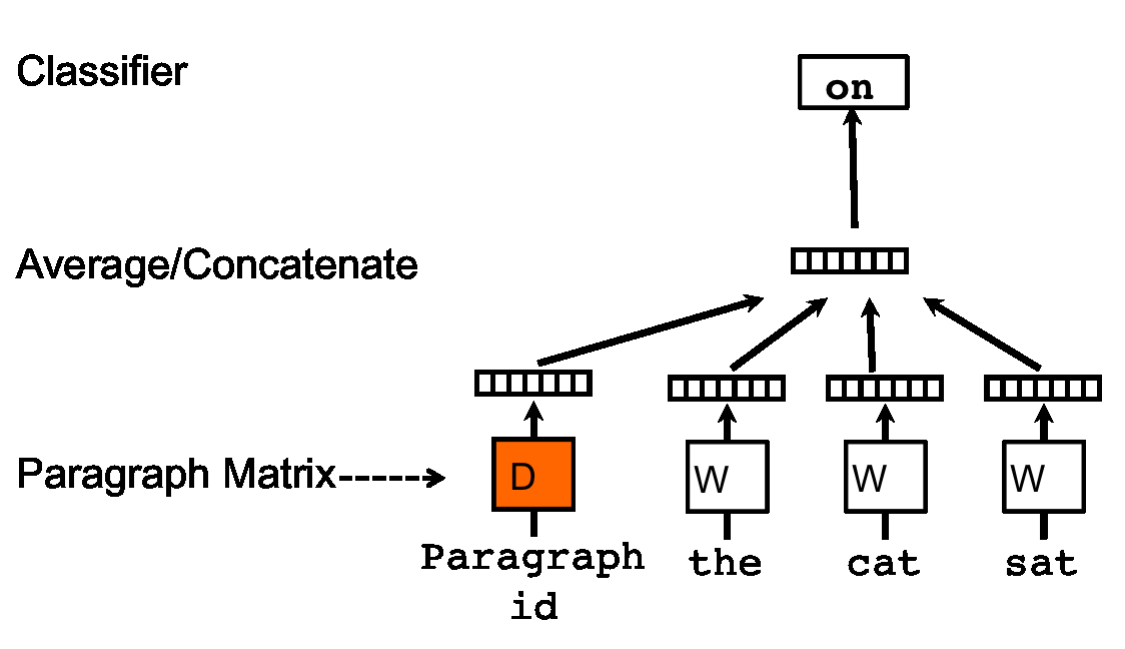
\includegraphics[scale=.6]{doc2vec}
    \caption{Doc2Vec Diagram\citep{le2014distributed}}
\end{figure}

Evaluating the "correctness" or accuracy of the embeddings presents a distinct challenge.  Unlike tasks where documents are classified for predefined categories (e.g., sentiment analysis), no such classification framework exists in our scenario.

To address this challenge, we employ a cosine similarity metric to generate a distance matrix that facilitates location comparisons.  For instance, we calculate the pairwise distances between all 500 restaurants within our dataset.  Ideally, if the resulting distances exhibit minimal variation, clustering these locations will likely be difficult.  Conversely, the presence of a significant range of distances indicates greater potential for successful cluster separation.

Doc2Vec incorporates two primary hyperparameters: vector size and window size.  Vector size determines the dimensionality of the generated vectors.  Smaller vectors limit the capacity to capture the variance between individual trip components.  Conversely, larger vectors require more computational resources for downstream tasks.  The window size defines the number of words considered before and after a target word when constructing embeddings.  Larger windows capture broader semantic relationships but come at a cost of increased computational intensity.  Generally, larger documents necessitate a larger window size.

With regards to vector size, we acknowledge that established embedding models like GloVe, trained on significantly larger datasets, utilize a vector size of approximately 300\citep{pennington-etal-2014-glove}.  Recognizing the more limited and focused nature of our data, we anticipated simpler embeddings.  Our experimentation revealed that a vector size of 100 coupled with a window size of 5 yielded sufficiently differentiated embeddings, enabling successful clustering of the transformed data.

For comparative purposes, consider the scenario where we employed "most mentioned words in reviews" metadata.  The corresponding cosine distances for each location pair exhibited minimal variation due to the prevalence of shared or similar high-frequency words across numerous locations.

\begin{figure}[H]
    \centering
    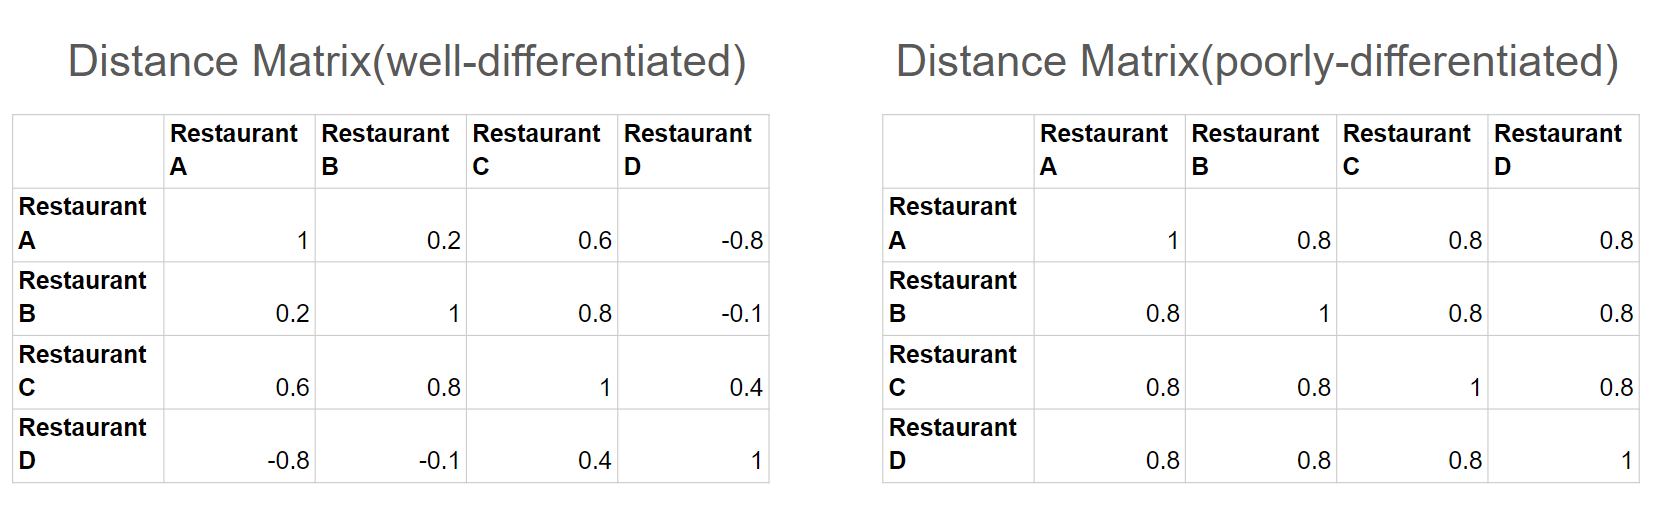
\includegraphics[scale=.8]{distancematrixex}
    \caption{Sample representative cosine-distance matrix for restaurant embeddings}
\end{figure}

The presence of distinct and varied cosine distances among many locations bolstered our confidence in the feasibility of successfully clustering these trip components. An additional sense check we conducted was to select at random an embedding, and use it to search our embedded database to see if the results were indeed similar to our query. For example, we would use the embedding for a fancy hotel as our query, and check if our response contained other similar fancy hotels.

\section{Clustering Evaluation and Methodology}

Having generated location embeddings, we now face the challenge of clustering these representations.  However, a key question emerges: how do we measure the "success" of our clustering efforts?  In this scenario, we lack pre-defined labels for each location.  Our objective is to establish user-interpretable groupings that align with potential user preferences.  Therefore, the primary evaluation method involves visual inspection of the resulting clusters to assess whether they exhibit some form of unifying characteristic (e.g., clusters are divided by cuisine/cost).  Ideally, a user would be amenable to exploring options within some particular clusters but less receptive to locations within other clusters.
We explored various clustering algorithms, including density-based, hierarchical, and partitioning-based approaches.  Our findings indicate that simple partitioning-based algorithms, such as K-means, are sufficient for achieving data separation and generating acceptable clusters.  While K-means offers advantages of computational efficiency and scalability, it necessitates pre-specification of the desired number of clusters.  As discussed below, this requirement does not pose a significant challenge in our case.

On the one hand, K-means necessitates the development of a specific strategy for determining the optimal number of clusters for each dataset, which can be a disadvantage.  On the other hand, this approach offers flexibility in adapting the number of clusters based on the unique characteristics of our data.  The size of our dataset allows for manual examination of clustering results and adjustments to the number of clusters without encountering unwieldy tasks.  However, for larger datasets, exploring methods for automated cluster number determination becomes more critical (addressed in the analysis section).

\subsection{Cluster Sizing Considerations}

We revisit our user requirements, specifically the constraint of a 5-minute timeframe for the initial user preference survey.  Given our dataset of 500 restaurants, 200 hotels, and 300 attractions, and assuming a survey limited to approximately 40 questions, a non-trivial challenge arises in dividing components across clusters.  Since cluster sizes can vary, we initially assume equal importance for each component category (restaurants, hotels, attractions).  This translates to an expected range of 10-15 questions per component category. Consequently, each category would ideally comprise 10-15 clusters.

This initial allocation might seem arbitrary at first glance. However, we reiterate that our objective is not to achieve "perfect" clusters.  Instead, we aim for sufficient data separation to yield user-interpretable groupings that potentially align with user preferences (such that a user selecting a particular cluster exhibits a preference for other items within the same group).  The precise boundaries between clusters hold less significance in this context.  While the possibility exists to identify points where better separation might occur with different cluster quantities, our findings (presented below) reveal that the chosen range of cluster numbers does not yield significant differences.


\begin{figure}[H]
    \centering
    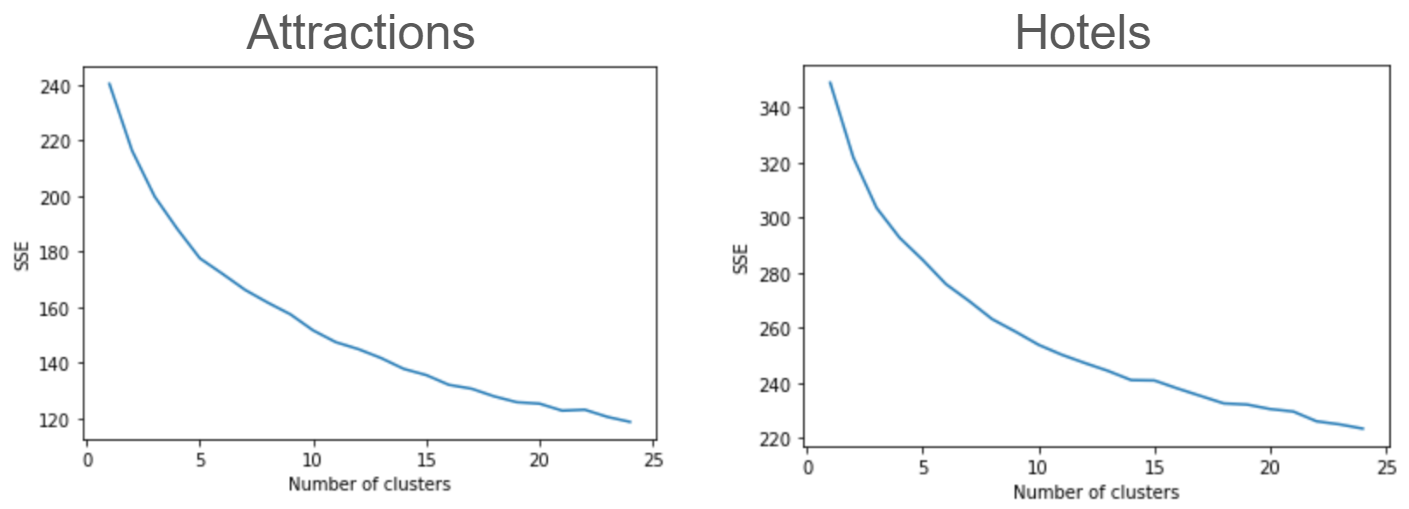
\includegraphics[scale=.8]{elbowcharts1}
    \caption{Error vs. number of clusters elbow charts for attraction and hotel embeddings}
\end{figure}

Visualizing high-dimensional clusters (100 dimensions and numerous clusters) using graph representations proves challenging.  Nonetheless, we present a few visualizations leveraging dimensionality reduction techniques.  Among these techniques, t-SNE emerges as the most successful compared to methods like PCA. The effectiveness of t-SNE stems from its ability to preserve semantic relationships between words or documents, facilitating more meaningful interpretations of the visualized clusters.  This stems from t-SNE's sensitivity to local relationships, which is crucial for capturing the nuances of human language\citep{JMLR:v9:vandermaaten08a}.

\begin{figure}[H]
    \centering
    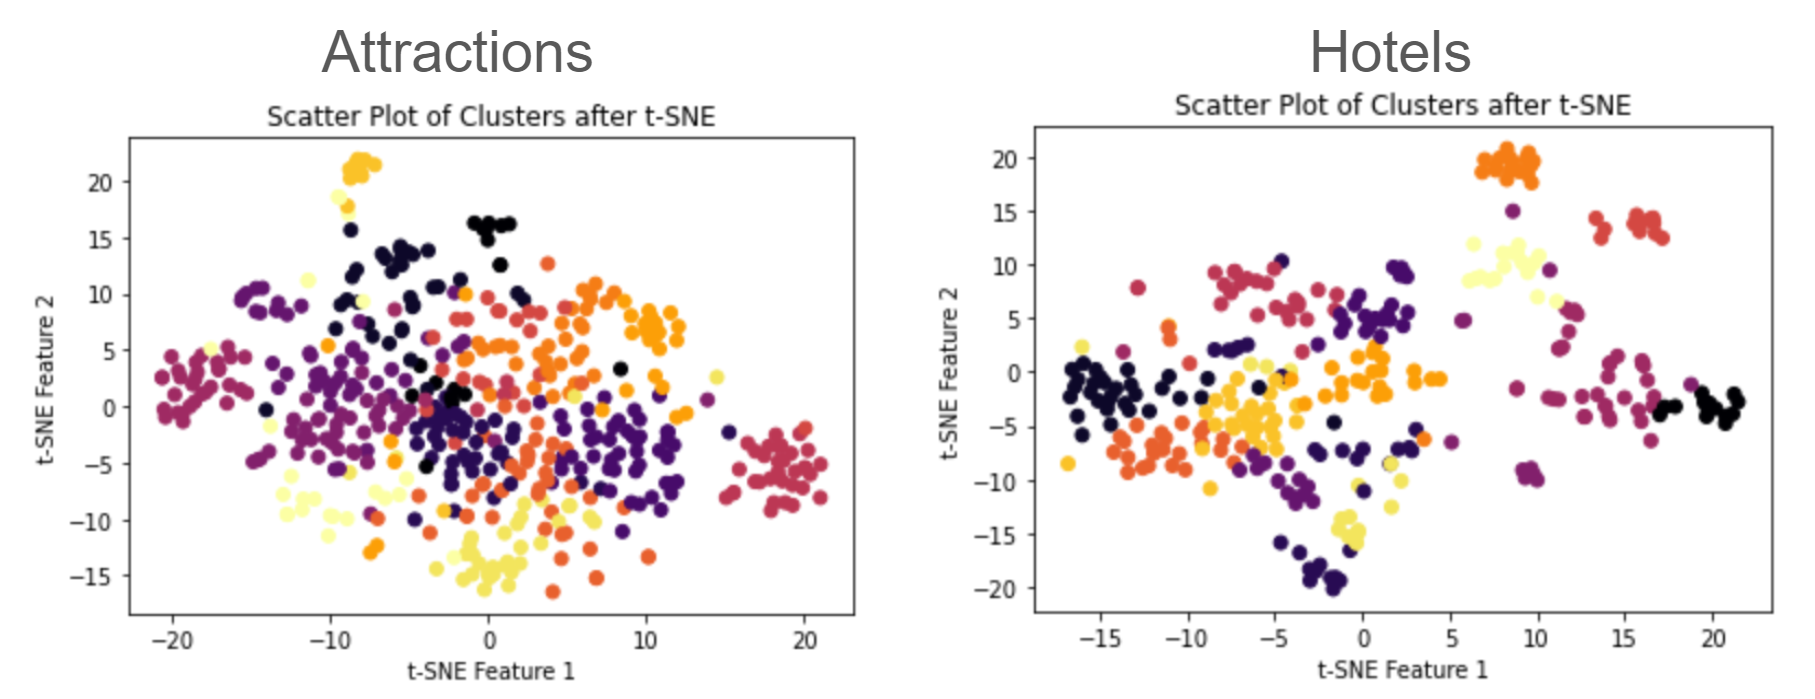
\includegraphics[scale=.6]{scatterplot1}
    \caption{Cluster visualization using t-SNE reduction for attractions and hotels}
\end{figure}

Human language inherently possesses a non-linear structure, often exhibiting complex relationships between words and concepts.  t-SNE effectively captures these non-linear relationships, while PCA might struggle with accurate representation.  Text data is also prone to outliers caused by typos, misspellings, or irrelevant information.  t-SNE exhibits greater resilience to outliers compared to PCA, enabling a more stable and interpretable visualization of clusters.

The visualizations confirm the success of our clustering efforts.  Among the restaurant clusters, we observe instances where a common theme is visually identifiable (e.g., Asian-themed cuisine, traditional tavernas, fine dining, bars).  Similar observations hold true for hotels (luxury accommodation, hostels, apartment rentals) and attractions (ancient ruins, quirky activities, shopping locations, walking tours).  These results support our hypothesis that clustering locations based on review content is not only feasible but also remarkably effective in capturing the unique "vibe" of a group of entities, a quality that can be challenging to describe discretely, even for humans.


\section{Post-Clustering Analysis and Survey Design}

Following the clustering process, we incorporate an additional column into our dataset for each trip component.  This column designates the cluster number to which each component belongs within its respective category (accommodation, restaurant, attraction).

Leveraging these clusters, we can now develop a user preference survey.  This survey is constructed by selecting a representative element from each cluster.  Our selection criterion prioritizes popularity within the cluster (measured by the number of reviews) over high ratings.  The rationale behind this approach is to capture the most representative archetype within each cluster.  For instance, within a cluster categorized as "ancient ruins," the Acropolis (the most famous Athenian archaeological site) would likely serve as a more effective illustration for users than a lesser-known but highly-rated tomb.  This approach aims to provide users with a clear understanding of the general type of travel component within the cluster.

\subsubsection{User Preference Survey Construction}
By selecting a single representative from each cluster, we can now construct a user preference survey.  This survey, comprising approximately 40 questions, utilizes a yes-or-no response format, prompting users with the question: "Does this look like something you'd want to do on a trip to Athens?"
In addition to the core preference questions, the survey also gathers essential trip parameters from users, including trip duration, number of attendees (adults/children), and a free-form section for listing additional requirements such as dietary preferences, accessibility needs, or other considerations.  The inclusion of a free-form response area for special user requirements allows us to potentially integrate these preferences directly into a large language model (LLM) for tailored itinerary generation.

\subsubsection{Survey Design Concerns}
Some weaknesses of this format are that it might be too lengthy for users to fill out, risking them abandoning the survey altogether. Another caveat is that we have elected a yes/no format for the survey responses for simplicity. The advantage to having a more granular scale rating system e.g. 1-5 could be that we could better differentiate a user's preferences. However, the drawback is that it may take even longer for a user to complete. 

\begin{figure}[H]
    \centering
    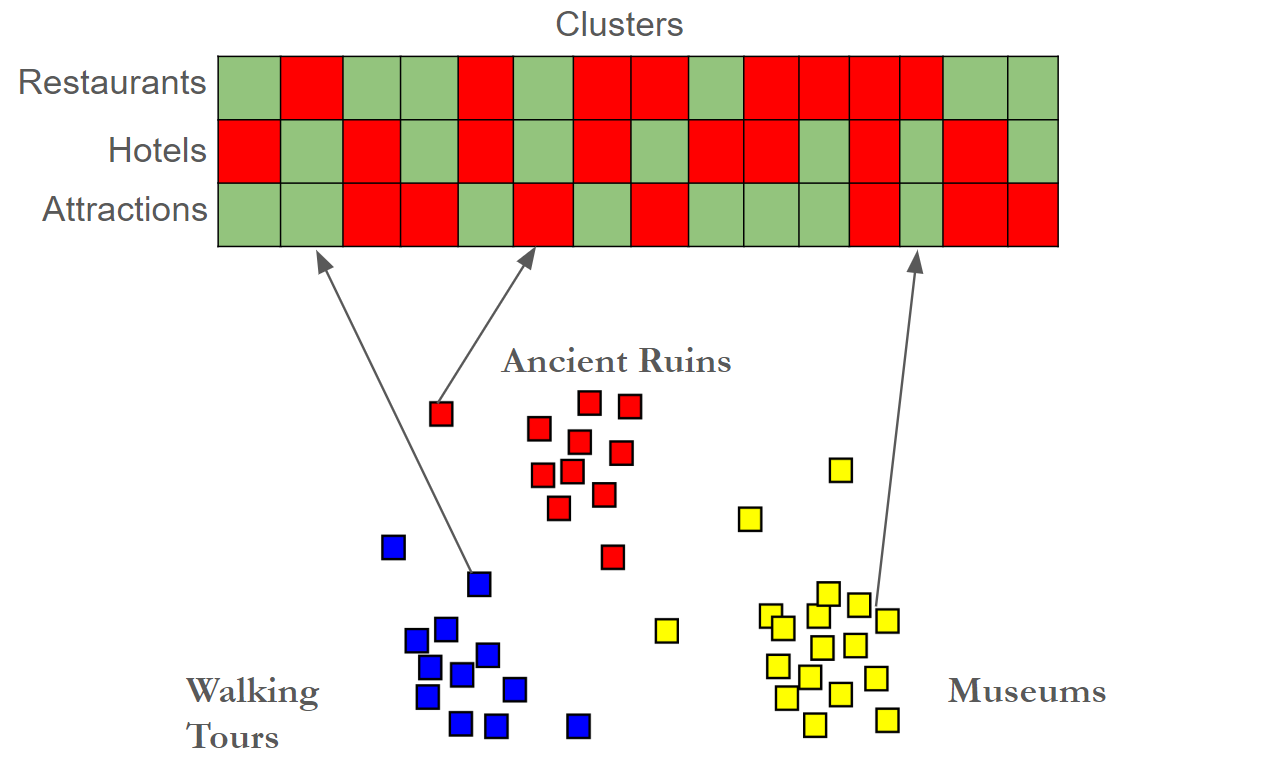
\includegraphics[scale=.6]{surveytoclusters}
    \caption{Survey response to cluster representative visualization: green/yes, red/no}
\end{figure}

This approach results in a potential $2^{40}$ unique customer profile combinations.

\section{Trip Component Candidate Selection}
Having successfully captured user preferences through the survey, we now possess knowledge of the user's preferred clusters.  Our next challenge involves assembling a candidate list of trip components while considering the overall trip duration.  Ideally, the generated list should offer a surplus of options compared to the minimum requirement, providing flexibility for the subsequent itinerary creation stage.  However, excessively extensive lists could potentially overwhelm a large language model during itinerary generation.

Therefore, we implement the following selection strategies for each trip component category:
\begin{description}
\item{\textbf{Accommodations:}  Given the specified location of Athens, users are likely to require accommodation at a single location throughout their trip.  However, hotels within Athens are situated across various neighborhoods, each offering a distinct ambiance that can influence itinerary structure.  For longer trips, a broader selection of hotels caters to itineraries with potentially dispersed activities.  Conversely, shorter trips necessitate a more limited(one or two) selection of hotels.}
\item{\textbf{Restaurants:}  Considering an average of three meals per day, the minimum requirement dictates the inclusion of at least three restaurant options per day (breakfast, lunch, dinner).  Furthermore, similar to the rationale for accommodations, we prioritize some degree of locational flexibility to optimize logistics.  Therefore, we opt to assemble a candidate list comprising five restaurants per day of the trip.}
\item{\textbf{Attractions:}  The duration of attraction visits can vary considerably, ranging from all-day excursions to brief museum visits.  Nevertheless, to provide users with ample choice, we aim to generate a list of at least four attractions per day of the trip.}
\end{description}
We now introduce the formal representation of the function that accepts user preferences as input and generates a list of candidate trip components as output.

\begin{lstlisting}[breaklines,breakatwhitespace,caption={Building Trip Component Candidates},label=Building Trip Component Candidates]

candidates = []
while len(candidates) <= trip_length * factor:
	for component in trip_components.orderedbypopularity:
		candidates += component 
\end{lstlisting}

The function iterates through each trip component category (accommodation, restaurant, attraction) and each user-preferred cluster.  Within each cluster iteration, the function progressively adds the highest-rated (or most popular) item to the candidate list until the maximum allowable number of components for that category is reached.  The maximum number of components is calculated by multiplying a scaling factor by the number of trip days.  For instance, a 3-day trip would result in a maximum of 15 restaurant candidates (3 days * 5 restaurants/day).  This process culminates in a comprehensive list of candidate trip components that serves as the foundation for itinerary generation.

\section{Itinerary Generation via Large Language Model}

Having assembled a candidate list of trip components, we can now proceed with itinerary generation.  Our initial approach involves presenting this list as input to a Large Language Model (LLM), along with a query requesting the creation of an itinerary that adheres to the specified user parameters.  An alternative approach would entail the development of a rule-based system.  Such a system would construct an itinerary from the ground up, leveraging information such as trip component descriptions and coordinates.  However, this method presents significant challenges in terms of complexity and scalability due to the inherent variability within collections of trip components, logistics, and inter-component distances.

We opted to utilize Google's Gemini LLM due to its position as a leading performer within the field of LLMs\citep{geminireport}.  Additionally, Gemini provides Application Programming Interface (API) access, facilitating efficient use case testing.  While open-source models represent a viable alternative, they might not achieve the same level of performance as Gemini.  Furthermore, open-source models might necessitate fine-tuning to optimize results.

\subsection{Prompt Engineering Considerations}

LLMs possess limitations regarding the amount of instruction they can effectively process.  To address this constraint, we adopted a "few-shot" approach, segmenting our user requirements across multiple prompts.  This strategy aims to increase the likelihood of generating a high-quality itinerary.  Typically, LLMs retain context by incorporating the content of prior queries and responses within subsequent interactions.  However, this context window is finite.  In the case of Gemini Ultra, which offers a comparatively extensive context window, this limitation is set at 32,000 tokens.  Each prompt typically consists of a few hundred tokens at most, providing a buffer zone.  This buffer is particularly important considering the potential need for future adjustments or content additions.

While we experimented with various hyperparameters, we ultimately employed the default settings for top-p, top-k, and temperature.  This decision ensured the consistent generation of coherent content aligned with the prompts.  In essence, we prioritized consistency over excessive LLM creativity in the hope of achieving improved performance based on our feasibility metrics. Below we give an example of an initial prompt, bearing in mind this is not visible to the user, rather submitted via API to the Gemini LLM.

\subsubsection{Prompt 1}
\textit{Hi, I would like to plan a unique and special itinerary for Me and my partner to Athens, Greece for 3 nights. There will be 2 adults and 0 children including myself. Can you please put together a detailed itinerary day-by-day that includes accommodations, meals and any other helpful suggestions? Here are some additional details as well - please pay special attention to these: I am vegan, but my partner is not. I want to experience the hidden spots in Athens, but also hit the main attractions. I am on a low budget, but happy to spend more on a few fancy experiences or dinners. I want a romantic dinner in a fancy restaurant on at least one night. I like rock music and shopping. I also need to get some souvenirs from my trip. . Do not forget to minimise travel distance, and explain transportation in detail too. If you mention to take a guided tour, you should suggest at least one specific guided tour company. I have narrowed down some of my favorite hotels, restaurants and activities below:HOTELS: The Athens Gate Hotel, Athens Green Apartments, Hermes Hotel, Plaka Hotel, Live in Athens, Short Stay Apartments, Acropolis Museum Boutique Hotel, Attalos Hotel, Athens Mosaico Suites Apartments, Philippos Hotel. RESTAURANTS: Avocado, Efcharis, Happy Blender, Maiandros, Smak, Arcadia Restaurant, Mama Tierra, Gods' Restaurant, Veganaki, Diodos Archaias Agoras, Yi, The Old Tavern of Psarras, Enjoy Just Falafel, ERGON House, Baba Ghanoush, Acropolis Museum Restaurant. ATTRACTIONS: Acropolis Museum, Plaka, Acropolis, National Archaeological Museum, Monastiraki, Parthenon, Benaki Museum - Museum of Greek Culture, Plateia Syntagmatos, Panathenaic Stadium, Museum of Cycladic Art, National Garden, Mount Lycabettus. Please make sure to give me 2 different hotel options to choose from. Make sure to state which restaurants or locations where we will eat. There must be a specific suggested restaurant for every meal. Give approximate travel time to/from each activity.}


We subsequently build upon this initial structure to incorporate additional details such as pricing and TripAdvisor links for each component.  Furthermore, we retain the results of the original preference survey as potential substitutes in case the LLM generates infeasible itinerary segments. We do find an initial drawback with such an extensive prompt where the LLM struggles to incorporate fully all details provided to it. For this reason, we find it more effective to use a few-shot approach to break down the requests step-by-step. Below we show a few further prompts that aim to further calibrate the resulting itinerary.

\subsubsection{Prompt 2}
\textit{"Keep the itinerary text and formatting as is, and make sure that method of transportation and how long it takes is given for every meal and activity. Optimize the itinerary to minimize travel distance by grouping activities/restaurants in a similar location. Make sure to include meals for breakfast, lunch and dinner. Make sure to mention a specific tour company for any tours. "}

\subsubsection{Prompt 3}
\textit{"Add the approximate costs for each activity and restaurant with a total estimate at the bottom. Don't forget any final adjustments to cater to the personal requests: I want a romantic dinner in a fancy restaurant on at least one night. I like rock music and shopping."}

The final output from the LLM represents the complete itinerary, which is then presented to the user.

\subsubsection{Output Itinerary}

\begin{figure}[H]
    \centering
    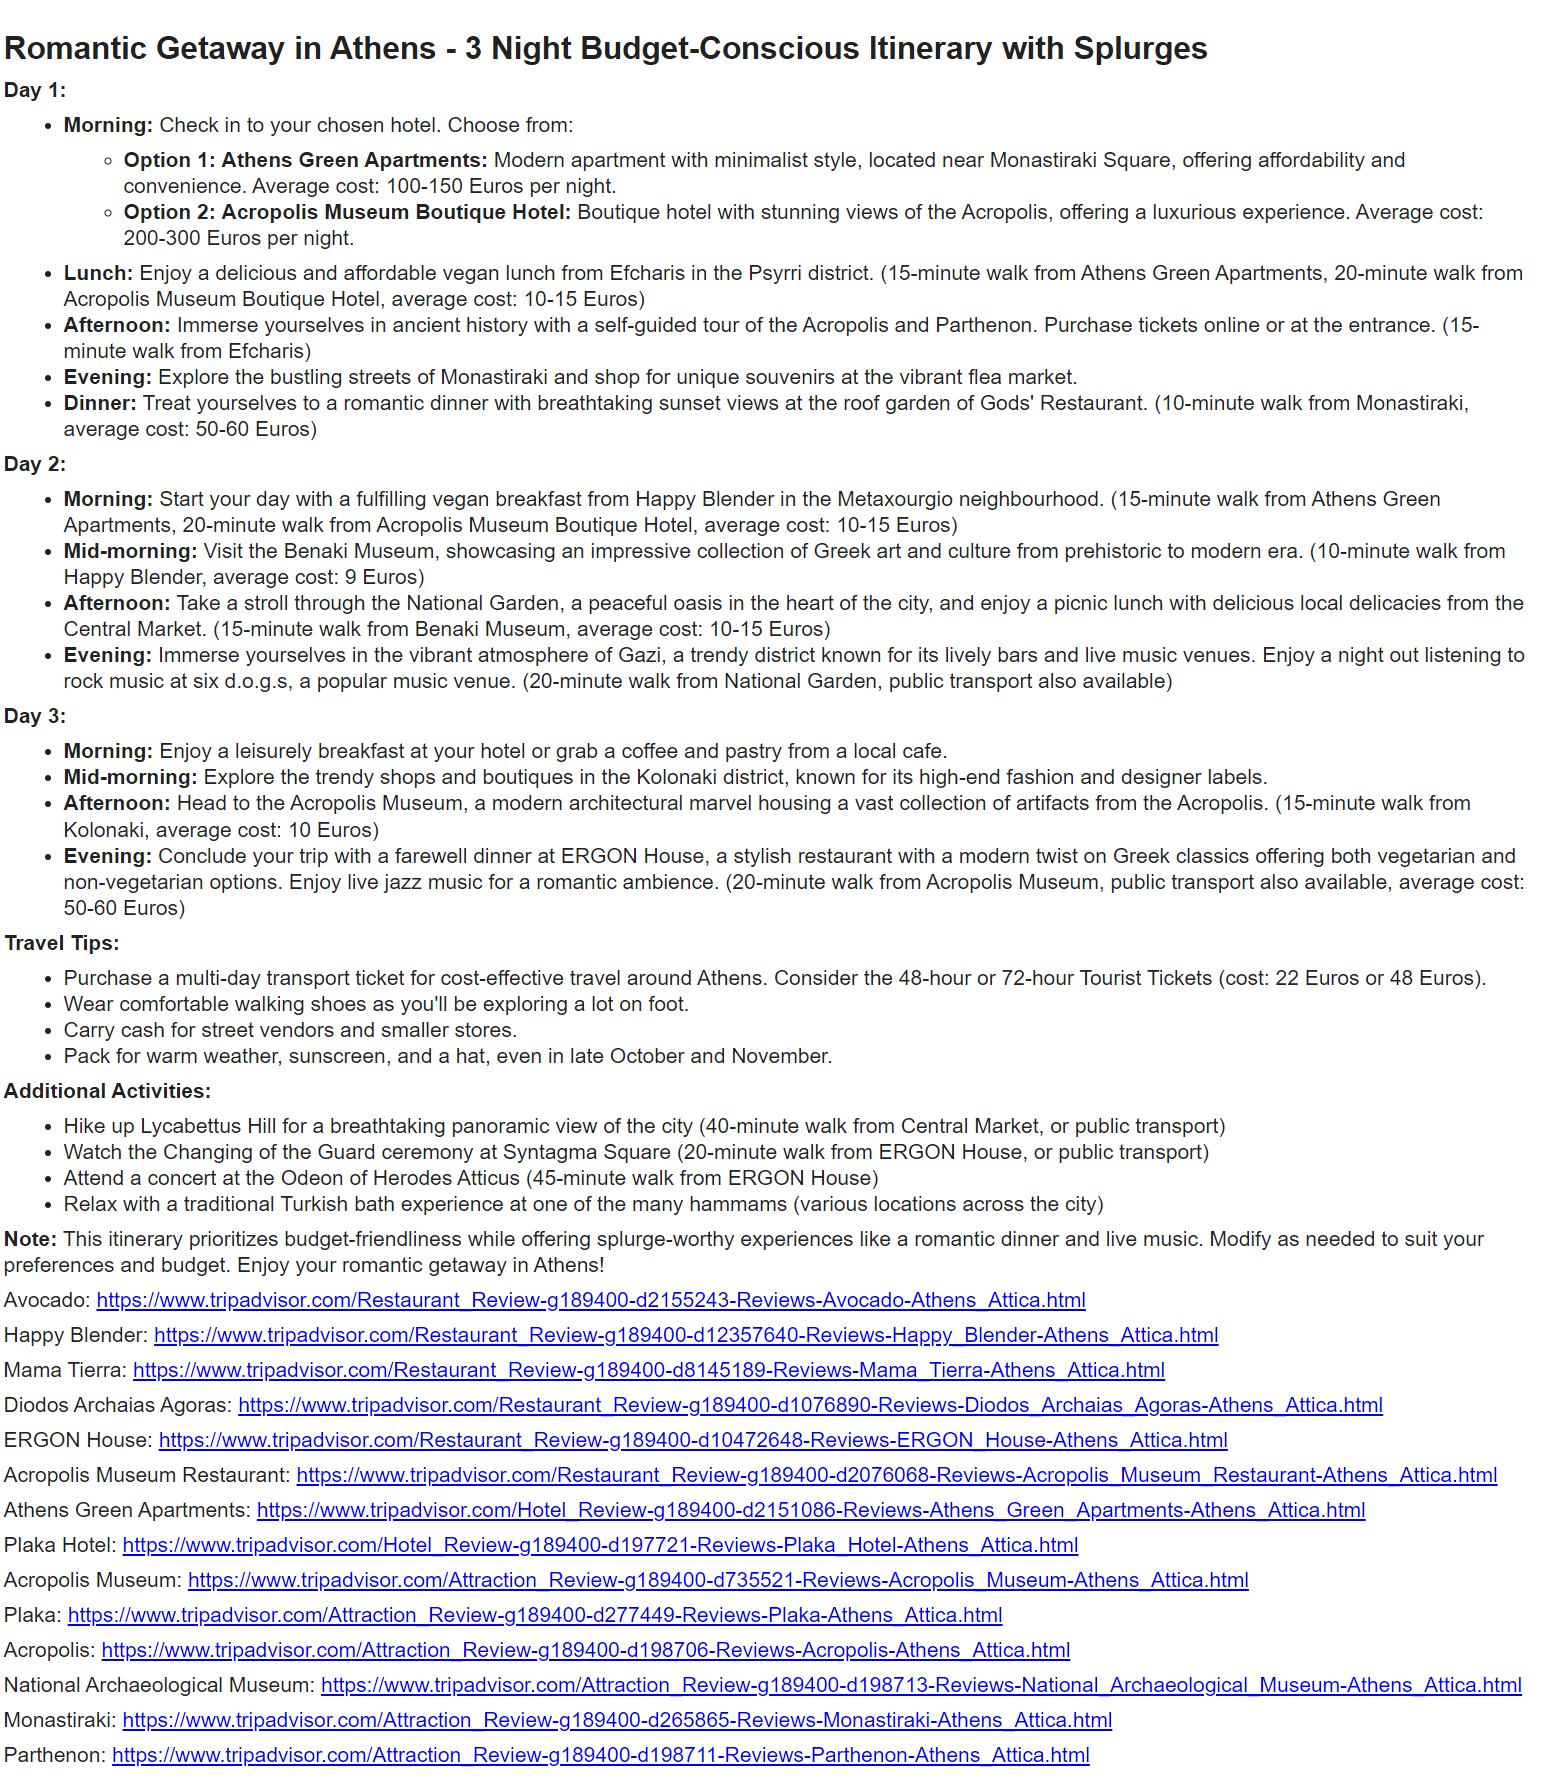
\includegraphics[scale=.8]{finalitinerary}
    \caption{Final Generated Itinerary}
   \label{fig:itinerary}
\end{figure}
%%%%%%%%%%%%%%%%%%%%%%%%%%%%%%%%%%%%%%%%%%%%%%%%%%%%%%%%%%%%%%%%%%%%%%%%%%%%%%%%
%%%%%%%%%%%%%%%%%%%%%%%%%%%%%%%%%%%%%%%%%%%%%%%%%%%%%%%%%%%%%%%%%%%%%%%%%%%%%%%%
\chapter{System and User Testing}


The proposed travel itinerary generation system comprises two primary stages: (1) clustering and embedding of travel component data, and (2) recommendation and itinerary generation. These stages operate asynchronously. Once the data preparation stage is complete and its output verified, the encoded data can be stored for high-confidence retrieval during itinerary generation. The testing and hyperparameter tuning process for the embedding and clustering modules is described in detail within the aforementioned methodology section.

This section focuses on the testing methodology employed for the itinerary generation module and the subsequent user feedback analysis.

\section{Itinerary Generation Requirements}

Our testing approach encompasses two key aspects: content/feasibility requirements and subjective user-facing requirements.

\subsection{Content Requirements}

\begin{enumerate}
\item{\textbf{Accommodation:} Each itinerary must include an accommodation option for every night.}
\item{\textbf{Food:} Restaurants or other food options (breakfast, lunch, dinner) should be suggested for each day.}
\item{\textbf{Activities:} Itineraries should incorporate at least one activity or point of interest for each day.}
\item{\textbf{Transportation:} Modes of transportation (public transport, taxi, etc.) for getting around should be specified.}
\item{\textbf{Costs:} Approximate costs for the aforementioned components should be provided.}
\end{enumerate}
These content requirements were evaluated using the following methodology. A set of random user profiles were generated, and the corresponding itineraries were reviewed to ensure they met all the specified criteria. Based on the results, prompts were adjusted or supplemented to enhance fulfillment of these requirements until satisfactory performance was achieved. Ideally, with more resources and time, a target reliability threshold (e.g., 95\% of generated itineraries meeting all criteria) could have been established in a setting where there are thousands of users. However, due to time constraints and the manual nature of the testing process (with a limited number of unique user profiles), testing concluded when the system consistently produced complete itineraries after 20 attempts.

\subsection{Feasibility Requirements}
\begin{enumerate}
\item{All travel components (restaurants, attractions, accommodations) must be verifiable and operational for user utilization.}
\item{Travel logistics and timeframes should be realistic and factual.}
\end{enumerate}

Feasibility requirements were tested in a similar manner to content requirements. Itineraries were generated based on randomly generated user profiles. However, verifying this aspect was significantly more challenging due to the need for manual investigation of unfamiliar components and transportation methods. This highlights the potential difficulty when scaling the system to locations beyond the initial test environment (e.g., Athens).

\subsection{User-Preferred Features}

Beyond objective content and feasibility, user satisfaction is a crucial factor. Here, we explore user-preferred features:
\begin{enumerate}
\item{\textbf{Personalized Content:} Itinerary content should align with user-specified preferences, including budget, activity type, cuisine, and desired ambience.}
\item{\textbf{Limited Customization Options:} Users should have the ability to make minor adjustments should certain aspects of the itinerary not align perfectly with their preferences.}
\end{enumerate}
These subjective user requirements necessitate direct user input. To this end, a concise user survey was developed for completion after receiving an itinerary. The survey aims to gauge user satisfaction, perceived level of personalization, and gather suggestions for improvement or additional features.

\section{User Survey Design}

Content requirements can be objectively evaluated. However, user preferences are inherently subjective, necessitating a large-scale user survey for comprehensive evaluation. To facilitate both quantitative and qualitative analysis, the survey incorporates both discrete answer options and open-ended questions.

\subsection{Quantitative Feedback}

\begin{enumerate}
\item{\textbf{Itinerary Rating:} Rate this itinerary on a scale of 1-10 (1 = unacceptable, 10 = perfect).}
\item{\textbf{Preference Reflection:} How well did the itinerary reflect your preferences (1-10)?}
\item{\textbf{Survey Length:} How was the length of the pre-itinerary preference survey (too long, too short, just right)?}
\item{\textbf{Recommendation Likelihood:} How likely are you to recommend this service to a friend/colleague (1-10)?}
\end{enumerate}

\subsection{Qualitative Feedback}
\begin{enumerate}
\item{What aspects of the itinerary did you find most appealing?}
\item{What aspects of the itinerary could be improved?}
\item{What single feature would you most like to see added?}
\end{enumerate}

%%%%%%%%%%%%%%%%%%%%%%%%%%%%%%%%%%%%%%%%%%%%%%%%%%%%%%%%%%%%%%%%%%%%%%%%%%%%%%%%
%%%%%%%%%%%%%%%%%%%%%%%%%%%%%%%%%%%%%%%%%%%%%%%%%%%%%%%%%%%%%%%%%%%%%%%%%%%%%%%%
\chapter{Results}

A generated itinerary is referenced in the methodology section and placed here \ref{fig:itinerary} for the reader.

\section{Content Requirement Evaluation}

Our evaluation confirms that the final system consistently fulfills the content requirements, including accommodation, food, activities, transportation, and cost information, for 100\% of generated itineraries. This is expected as our prompts explicitly instruct the model to generate itineraries adhering to this format. The reliability of content generation in response to specific prompts is well-established. However, the quality of the content itself remains a more critical aspect of Large Language Model (LLM) output. Interestingly, content loss only occurs when excessive subsequent prompts are introduced. In such cases, the model prioritizes the most recent prompt, neglecting the original task. This can be readily addressed by incorporating instructions within subsequent prompts to preserve the initial context.

\section{Feasibility Requirement Evaluation: Travel Components}

This section analyzes the system's performance in meeting feasibility requirements, which stipulate that all suggested travel components (restaurants, attractions, accommodations) must be operational and accessible to users. Furthermore, travel logistics and timeframes should be realistic.

\subsection{Travel Component Existence and Availability}

The existence and operational status of travel components heavily depend on the quality of the input data. In our case, TripAdvisor reviews were used. While rare, instances occurred where a component, such as the Hilton Athens undergoing renovation, was suggested despite being temporarily closed. This highlights a limitation: the model relies on the provided data and doesn't account for dynamic changes like seasonal closures. Although including seasonal instructions within prompts could be explored, time constraints prevented testing its effectiveness in this proof-of-concept.

However, the model successfully categorized restaurants for different meals. For example, cafes with breakfast options were suggested for mornings (often including the option to eat at the hotel), while traditional tavernas or "dinner" options were chosen for evenings. This is expected behavior as Gemini is trained on a vast dataset including numerous travel itineraries, likely encompassing Athens, a popular tourist destination.

Integrating Google Maps data, known for its accuracy regarding opening hours, could be a future improvement. However, computational cost becomes a factor depending on the chosen update frequency (risk tolerance). Since most locations experience infrequent changes in operating hours, we believe this approach is feasible.

\subsection{Travel and Logistics}

Here, we evaluate the itinerary's accuracy in representing travel times and overall logistics. This area revealed a clear weakness in the LLM's ability to construct itineraries, potentially posing one of the most significant challenges for future development.

Some generated itineraries displayed inaccuracies. For instance, a user might be instructed to "walk 5 minutes" to a location that was actually a 20-minute car ride away. Similarly, implausible scenarios emerged, such as suggesting a day trip to a location over an hour away by car, yet  including lunch at a restaurant still within the city center. Such errors, if acted upon, could cause significant inconvenience and stress for unsuspecting travelers.

Furthermore, explicit instructions to the LLM to optimize travel distance and time or verify logistics information proved ineffective. The model was unable to identify these issues as exemplified below:

\textit{Dinner: Have a traditional Greek meal at Psomi and Alati near the Acropolis (approx. €20; \textbf{15 min. walk).}}

\begin{figure}[H]
    \centering
    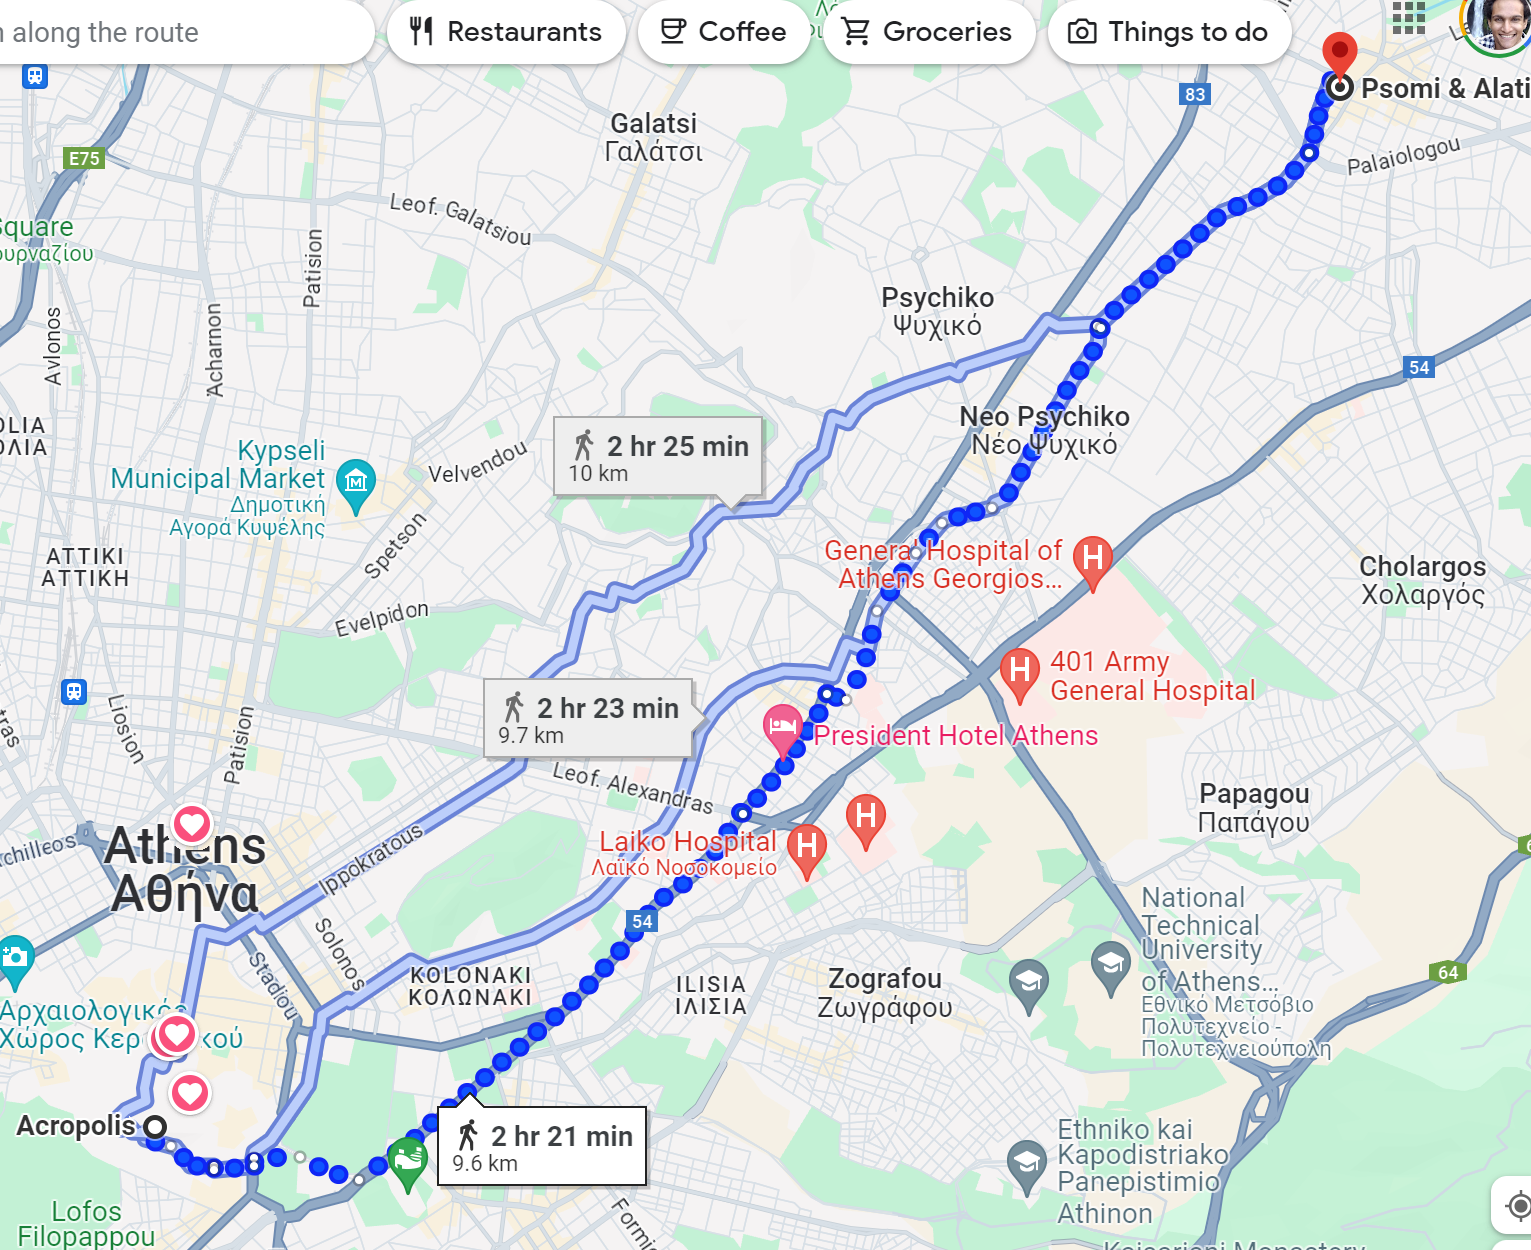
\includegraphics[scale=.55]{mapfail}
    \caption{Google Map directions for alleged 15 minute walk}
\end{figure}

While challenges exist, all is not lost. Path optimization is a computationally complex problem, and expecting an LLM to find an optimal graph solution is unrealistic. Our goal is not absolute optimization but rather eliminating disastrous recommendations.

One potential solution involves restricting suggested travel components to a predefined distance radius. This approach, however, could limit access to certain key points of interest.

Another recent development involves Google's integration of Google Maps into its LLM infrastructure when prompted appropriately. This allows the model to access actual distances between locations. However, understanding and implementing this knowledge appears to be a bigger hurdle for current LLMs. For instance, a prompt requesting the distance between two locations might successfully trigger Google Maps integration, providing an accurate response. Yet, in cases where this integration fails, a null response or an inaccurate hallucination directly from the LLM is highly likely.

Finally, training and fine-tuning a custom LLM specifically designed for tourism tasks could potentially mitigate these "hallucinations." This approach will be further explored in the "Future Applications" section.

\section{User Feedback}

This section presents the findings from a user feedback survey, where all numerical ratings were based on a 10-point scale.

\subsection{Quantitative Feedback}

The overall user response was positive. The average itinerary rating was \textbf{8.8}, indicating a high level of user satisfaction. Similarly, users felt the itineraries reflected their preferences with an average score of \textbf{9.2}. The likelihood of recommending the service to others received an average score of \textbf{8.8}.

\subsection{Qualitative Feedback}

Qualitative responses echoed the positive sentiment and highlighted potential areas for improvement, which align with known limitations. Below we give a few examples of verbatim feedback.

\subsubsection{Positive Feedback}

Alignment with user preferences: “Most of the activities are spot on for what I'd want to be doing… many of the recommendations… align with what I enjoyed.” This suggests the system effectively personalizes itineraries based on user input. 

\subsubsection{Feature Requests}
\begin{description}
\item{Annotated maps: “Provide an annotated map.” Integrating annotated maps within the itinerary could enhance user experience and visual comprehension.}
\item{User-driven modifications: “Communicate desired changes back to the system at the end.” Enabling users to suggest modifications directly within the system would streamline the feedback loop and improve itinerary refinement.}
\item{Cost summary: “Also, summary of total cost at the end.” Providing a consolidated cost summary would enhance transparency and user planning.}
\item{Direct booking links: “Direct booking links.” Integrating direct booking links would increase functionality and potentially streamline the user experience.}
\end{description}

\subsubsection{Limitations of User Feedback}

The user feedback process does have some limitations:

\begin{description}
\item{\textbf{User Attentiveness:} Users don’t always check every line of the itinerary thoroughly. This highlights the potential for users to overlook details within the itinerary.}
\item{\textbf{Hypothetical Scenario:} Since users don’t actually use the itinerary in this scenario, the whole thought process is hypothetical. The survey focused on hypothetical usage, potentially neglecting practical considerations that might arise during an actual trip.}
\item{\textbf{Potential Bias:} Selection criteria of the users was merely sent out to friends and acquaintances who may be more inclined to give positive feedback. The use of non-random participants could introduce bias towards positive feedback.}
\item{\textbf{Public User Interface (UI):} Due to time and technical constraints, it was not possible create a public facing UI. Developing a public UI would allow for wider user testing and more comprehensive feedback collection.}
\item{\textbf{User Feedback Loop Integration:} Integrating a user feedback loop within the system would allow for iterative refinement based on user input.}
\end{description}
In the next section, we further conduct an analysis of these results and propose areas for future work.

%%%%%%%%%%%%%%%%%%%%%%%%%%%%%%%%%%%%%%%%%%%%%%%%%%%%%%%%%%%%%%%%%%%%%%%%%%%%%%%%
%%%%%%%%%%%%%%%%%%%%%%%%%%%%%%%%%%%%%%%%%%%%%%%%%%%%%%%%%%%%%%%%%%%%%%%%%%%%%%%%
\chapter{Critical Evaluation}


\section{Model Achievements and Evaluation}

Our work presents the first fully-automated, personalized travel itinerary generation system with encouraging initial user feedback from a limited sample. The system leverages existing travel data and the capabilities of state-of-the-art LLMs to create personalized itineraries for Athens, Greece, with the potential for scalability to other destinations.

We successfully achieved our content requirements, generating comprehensive itineraries that include attractions, accommodations, and food options for nearly all user trials. User feedback was generally positive, with few criticisms and high ratings for personalization and recommendation value. Most users indicated a willingness to recommend the system to others.

\section{Data Engineering Considerations}

Our initial data engineering approach involved clustering trip components (e.g., restaurants) based on user reviews, with the expectation of creating well-defined clusters that align with user preferences (e.g., cuisine type for restaurants). The number of clusters was determined based on a trade-off between downstream user survey complexity and achieving well-separated clusters.

A key limitation of this approach is its manual nature.  While it may be suitable for this Athens prototype, it likely wouldn't scale effectively to other cities without significant adjustments. Additionally, there is no guarantee that this method will always produce "good" clusters. Automating the number of clusters based on user input volume is a possibility, but the system, in its current form, would still require re-evaluation and potentially re-clustering for each new travel destination.

Furthermore, while the source data is unlikely to change dramatically in the short to medium term, long-term data refresh is likely necessary as travel components evolve (businesses open or close, activities change). This would necessitate re-evaluating clusters, impacting downstream processes like user input and itinerary generation. These challenges are surmountable but require careful consideration for sustainable system growth.

\section{LLM Hallucination and Future Applications}

The most significant challenge encountered was meeting all logistical requirements perfectly. In some instances, the LLM struggled to accurately represent distances and logistics between points of interest. We anticipated this potential issue when opting for an LLM due to its human-like language capabilities. However, model hallucination, resulting in non-factual information, remains a significant hurdle. In domains requiring precise information, LLMs might be a questionable choice despite their powerful generation abilities.

Despite this shortcoming, users still found value in the system's ability to generate personalized recommendations. The system significantly reduces travel search time and provides users with the opportunity to visualize potential itineraries tailored to their preferences.

While a rule-based system could have been a design option, the complexity of building such a system to handle intricate travel logistics in a piecemeal fashion outweighs the limitations introduced by occasional LLM hallucinations.  Perhaps a more appropriate positioning for this tool is as a travel visualization and search aid, rather than a comprehensive itinerary planner. Additionally, travel agents could potentially leverage this tool to streamline itinerary creation for their clients.

\section{Additional Implemented Features Based on User Feedback}

User feedback informed the incorporation of several new features:

\begin{description}
\item{\textbf{Pricing}: Users requested approximate pricing for itinerary components (restaurants, hotels, tours) and a total trip cost estimate. While fetching exact prices is difficult due to their dynamic nature and dependence on unknown user preferences (e.g., room type), we can leverage a combination of TripAdvisor data and LLM estimates to provide reasonably accurate costs during itinerary generation.}
\item{\textbf{Links:} Users requested web links for all trip components, facilitating further exploration and verification. This feature was straightforward to implement, involving fetching associated links from our database and appending them to the itinerary during generation.}
\item{\textbf{Alternatives:} Users desired options beyond a single choice for restaurants, accommodations, etc. This feature enhances the user experience by providing a broader view of available options. However, introducing alternatives can create feasibility challenges due to potential distance discrepancies. For example, an alternative accommodation far from the initial suggestion might necessitate significant itinerary adjustments. We mitigate this by instructing the LLM to prioritize alternatives within the same area, although this limits the generation of entirely different itineraries.}
\end{description}

\section{Comparison to Baseline ChatGPT(and other baseline LLMs)}

A qualitative comparison with an unmodified ChatGPT itinerary highlights the advantages of our system. While ChatGPT can generate itineraries, they lack personalization and are not directly linked to a database, resulting in the absence of specific locations, prices, or links. Although ChatGPT might be a useful starting point for trip planning, it necessitates further research on travel platforms like TripAdvisor or Google Maps. Conversely, our system provides detailed, personalized itineraries with activities, restaurants, accommodations, prices, and alternatives, significantly reducing user search time.


%%%%%%%%%%%%%%%%%%%%%%%%%%%%%%%%%%%%%%%%%%%%%%%%%%%%%%%%%%%%%%%%%%%%%%%%%%%%%%%%
%%%%%%%%%%%%%%%%%%%%%%%%%%%%%%%%%%%%%%%%%%%%%%%%%%%%%%%%%%%%%%%%%%%%%%%%%%%%%%%%
\chapter{Future Work}


This project represents a proof-of-concept prototype with limitations imposed by time and resource constraints. Nevertheless, we envision a multitude of potential improvements and functionalities that could significantly enhance the user experience in trip planning. These advancements are categorized based on user interaction points.

\section{User Preference Ingestion}

Our current system relies on user responses to a series of yes/no questions corresponding to trip component clusters. The number of questions directly correlates with the number of clusters, which can vary by location. To streamline this process for future iterations, we propose the following:
\begin{description}
\item{\textbf{User-based Recommendation:} As our user base grows, we can leverage user preference data to make inferences. If a critical mass of users enjoys Cluster X in Location 1 and Cluster Y in Location 2, and a new user has also visited Location 1 and liked Cluster X, we can infer a potential preference for Cluster Y in Location 2. This reduces the need for explicit user input in such scenarios. With a substantial user base, gathering preferences might become unnecessary if sufficient user profiles with similar travel interests exist.}
\item{\textbf{Uncorrelated Elimination:} Each trip component is stored as an embedding, a vector that allows us to calculate cosine distance from other components. If a user expresses a preference for a specific cluster (e.g., luxury hotels), we can eliminate clusters with significantly different cosine distances (e.g., hostels, budget hotels). However, this approach risks excluding viable options, as some clusters are not mutually exclusive (e.g., Indian restaurants and traditional Greek tavernas). Nonetheless, a method likely exists to reduce user input requirements based on cosine distance analysis.}
\end{description}

\section{LLM Refinement}
\begin{description}
\item{\textbf{Hyperparameter Tuning:} We acknowledge the potential benefits of further exploration with LLM hyperparameters (top-p, top-k, temperature) to generate more creative, yet potentially less accurate, content. This could be an intriguing user feature for sparking travel inspiration.}
\item{\textbf{Interactive LLM Interface:} A highly requested feature is the ability to edit and adjust itineraries after generation. Ideally, this would involve a direct interface with an LLM, similar to publicly available services like ChatGPT or Google's Gemini. While technically possible with our current implementation, the broad training of these LLMs makes them less suitable for our specific use case.}
\item{\textbf{Travel-Specific LLM:} Training a travel-specific LLM to act as a "virtual travel agent" for user interaction would offer several advantages. It would minimize potential issues like user queries for unrelated information or leakage of sensitive data. Additionally, training this LLM on travel-specific data (descriptions, itineraries) could improve itinerary generation quality and potentially reduce long-term resource costs by creating more in-depth and detailed itineraries in a single run, as opposed to our current multi-prompt approach. The development of a travel-specific LLM is resource-intensive, but the potential benefits are significant. Furthermore, a travel-specific LLM trained on itinerary data might minimize current model weaknesses related to hallucination.}
\end{description}

\section{Data Source Integration}

Our current model relies solely on TripAdvisor data. Here are potential data sources for future iterations:
\begin{enumerate}
\item{\textbf{Google Maps Data:} Google Maps offers location-based data on trip components (restaurants, accommodations, attractions) similar to TripAdvisor. Including this data could enrich our clustering and itinerary generation while reducing potential data bias.}
\item{\textbf{Travel Blogs and Websites:} Travel planning often involves consulting various sources beyond Google Maps and TripAdvisor. A wealth of travel blogs, adventure companies, guides, and personal websites offer valuable insights and even complete itineraries. Incorporating this data as training material for an LLM could be instrumental in capturing unique and complex travel experiences, and enhancing user discovery. Harvesting and scraping trip component data from these sources presents challenges but is a vital aspect of the project's data strategy.}
\item{\textbf{Global Expansion:} While our prototype focused on Athens, Greece, we envision expanding the model to encompass other locations globally, particularly data-rich urban areas. Exploring the incorporation of non-English language data is also a future possibility.}
\end{enumerate}
\section{API Integration}

Our current model utilizes a database to retrieve user information. However, users have requested features that would necessitate API integration:

\begin{enumerate}
\item{\textbf{Real-Time Availability:} Users desire the ability to view real-time availability of various trip components and potentially initiate bookings directly from the platform. APIs from booking platforms could be integrated to address this need.}
\item{\textbf{Interactive Maps:} Integrating a virtual map with highlighted recommendations would significantly enhance the planning and exploration process. Since we already leverage location data from Google Maps and TripAdvisor, incorporating this feature would be relatively straightforward.}
\item{\textbf{Flight and Hotel Booking:} Several platforms (e.g., Google Flights, SkyScanner, Booking.com, Airbnb) offer real-time flight data, pricing, and booking APIs. Integrating these APIs would allow our system to provide users with flight and hotel options directly.}
\end{enumerate}

Overall, we look forward to bringing these features, modifications, and improvements to life in future versions of our model. 

%%%%%%%%%%%%%%%%%%%%%%%%%%%%%%%%%%%%%%%%%%%%%%%%%%%%%%%%%%%%%%%%%%%%%%%%%%%%%%%%
%%%%%%%%%%%%%%%%%%%%%%%%%%%%%%%%%%%%%%%%%%%%%%%%%%%%%%%%%%%%%%%%%%%%%%%%%%%%%%%%
\bibliography{ExampleBibFile}

%%%%%%%%%%%%%%%%%%%%%%%%%%%%%%%%%%%%%%%%%%%%%%%%%%%%%%%%%%%%%%%%%%%%%%%%%%%%%%%%
%%%%%%%%%%%%%%%%%%%%%%%%%%%%%%%%%%%%%%%%%%%%%%%%%%%%%%%%%%%%%%%%%%%%%%%%%%%%%%%%
\appendix

%%%%%%%%%%%%%%%%%%%%%%%%%%%%%%%%%%%%%%%%%%%%%%%%%%%%%%%%%%%%%%%%%%%%%%%%%%%%%%%%
%%%%%%%%%%%%%%%%%%%%%%%%%%%%%%%%%%%%%%%%%%%%%%%%%%%%%%%%%%%%%%%%%%%%%%%%%%%%%%%%
\chapter{Design Diagrams}

\begin{figure}[H]
    \centering
    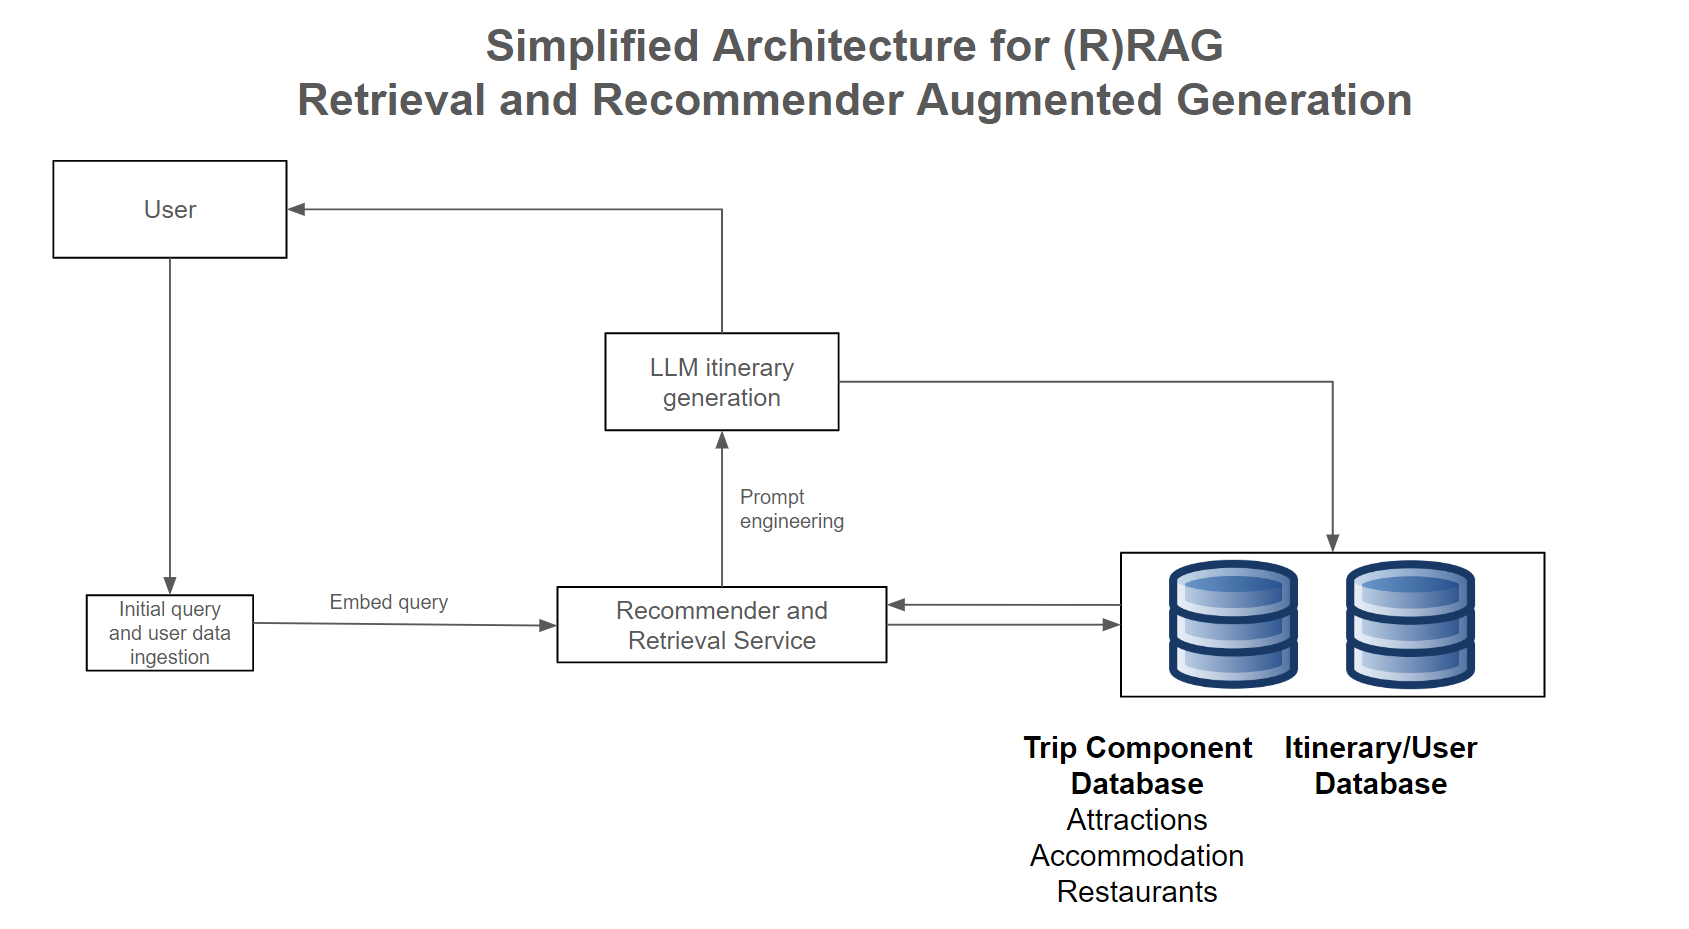
\includegraphics[scale=.7]{systemdiagram}
\end{figure}

\begin{figure}[H]
    \centering
    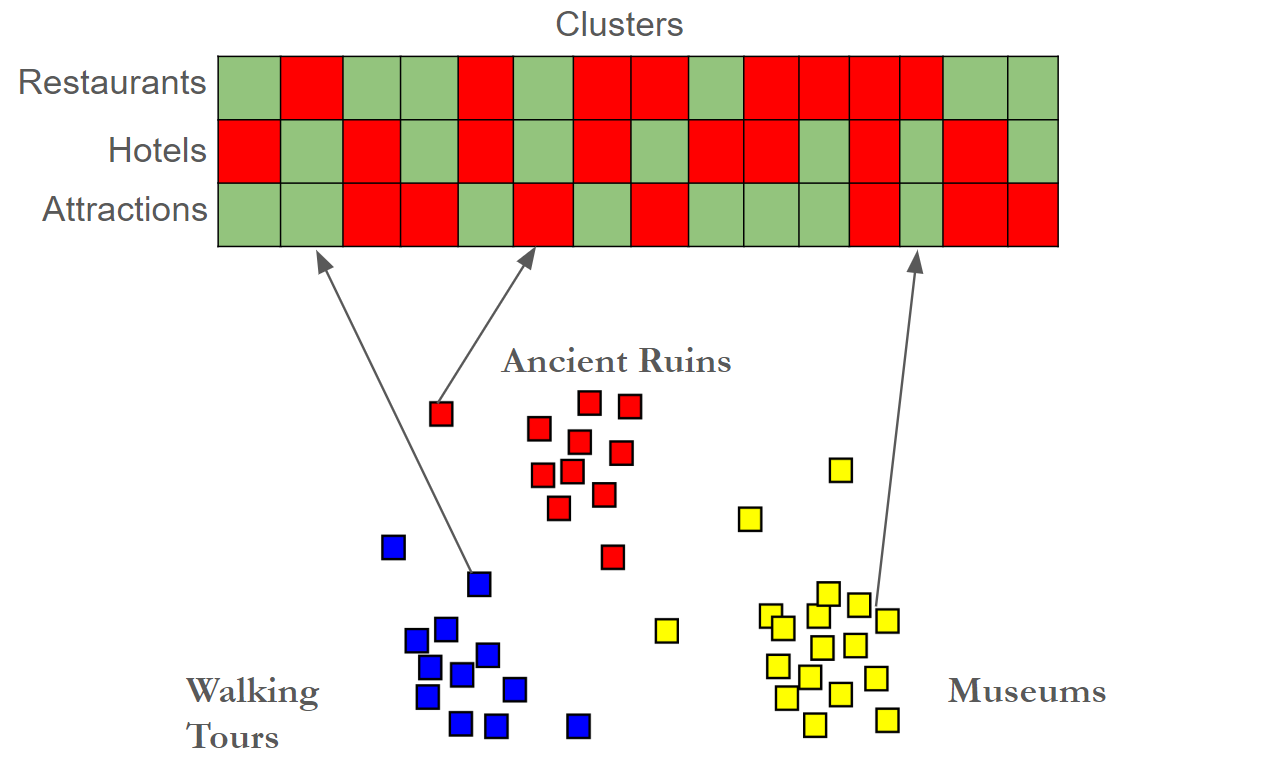
\includegraphics[scale=.6]{surveytoclusters}
    \caption{Survey response to cluster representative visualization: green/yes, red/no}
\end{figure}

%%%%%%%%%%%%%%%%%%%%%%%%%%%%%%%%%%%%%%%%%%%%%%%%%%%%%%%%%%%%%%%%%%%%%%%%%%%%%%%%
%%%%%%%%%%%%%%%%%%%%%%%%%%%%%%%%%%%%%%%%%%%%%%%%%%%%%%%%%%%%%%%%%%%%%%%%%%%%%%%%
\chapter{Sample Itineraries}
\begin{figure}[H]
    \centering
    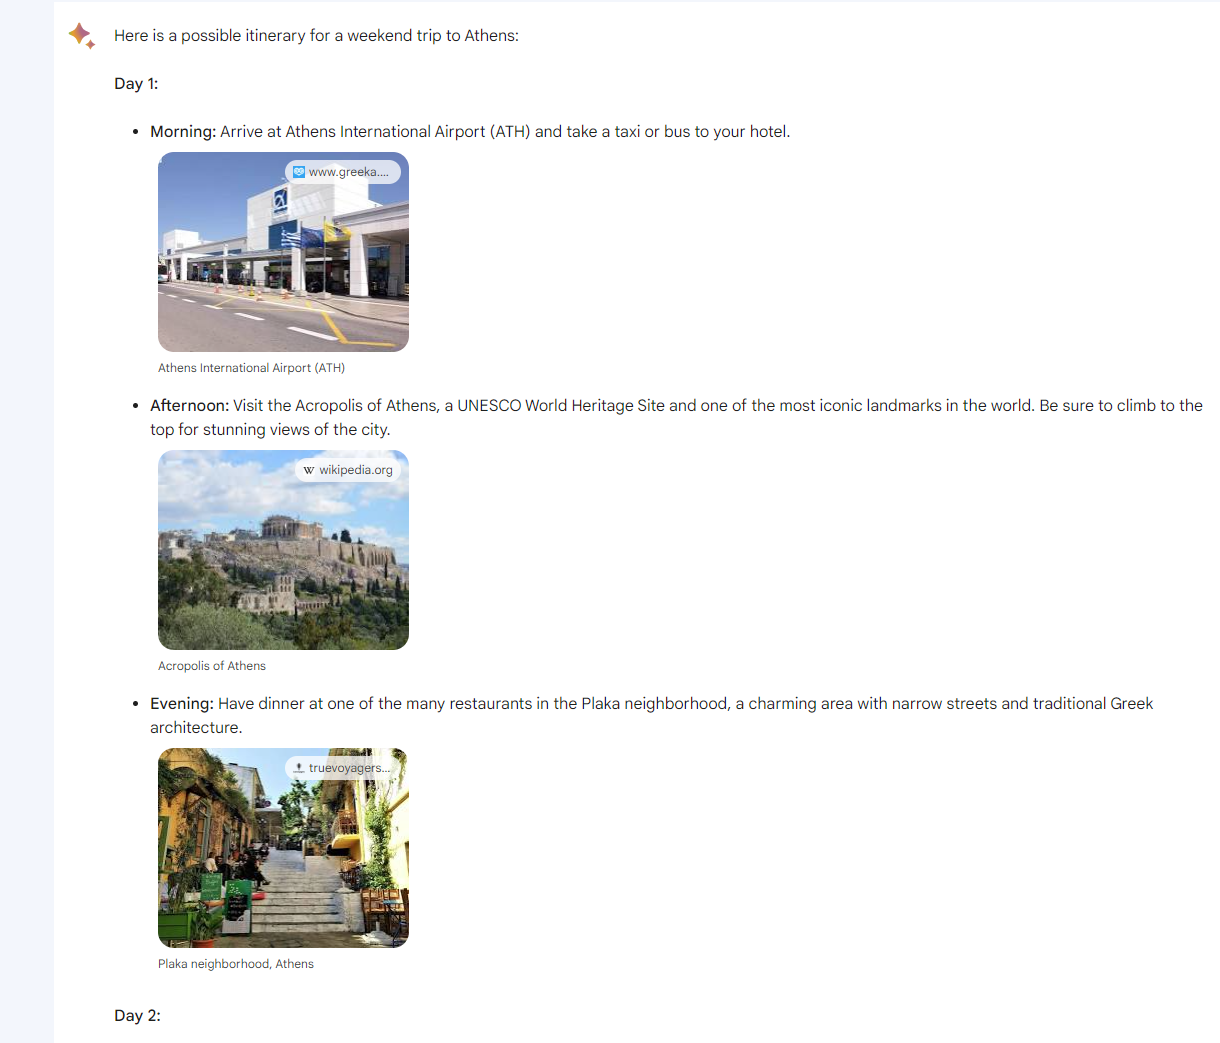
\includegraphics[scale=.5]{athensbardexample}
    \caption{Athens Itinerary by Google's Bard LLM}
\end{figure}

\begin{figure}[H]
    \centering
    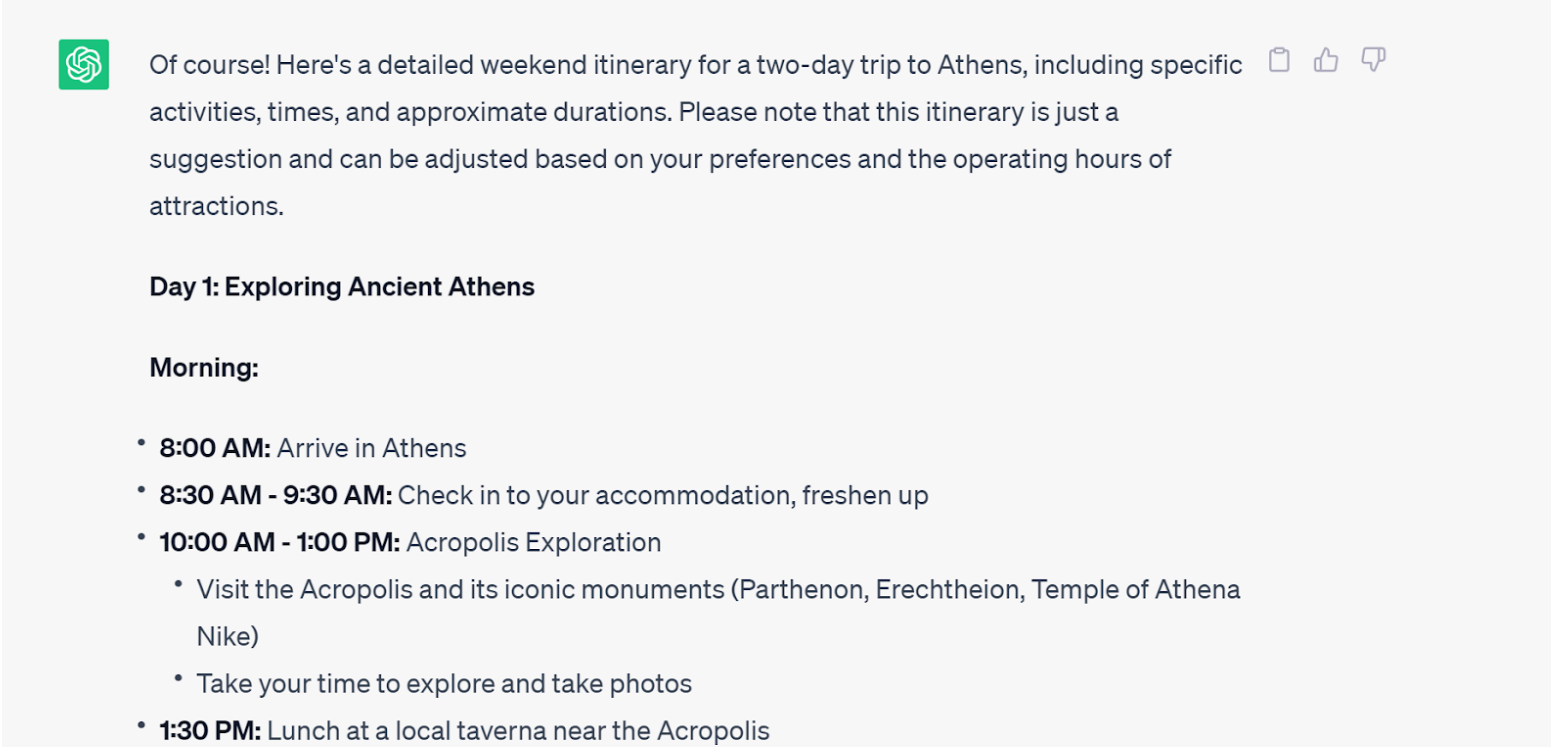
\includegraphics[scale=.8]{chatgptitin}
    \caption{Athens Itinerary by OpenAI's ChatGPT}
\end{figure}
%%%%%%%%%%%%%%%%%%%%%%%%%%%%%%%%%%%%%%%%%%%%%%%%%%%%%%%%%%%%%%%%%%%%%%%%%%%%%%%%
%%%%%%%%%%%%%%%%%%%%%%%%%%%%%%%%%%%%%%%%%%%%%%%%%%%%%%%%%%%%%%%%%%%%%%%%%%%%%%%%
\chapter{Raw Results Output}

\begin{figure}[H]
    \centering
    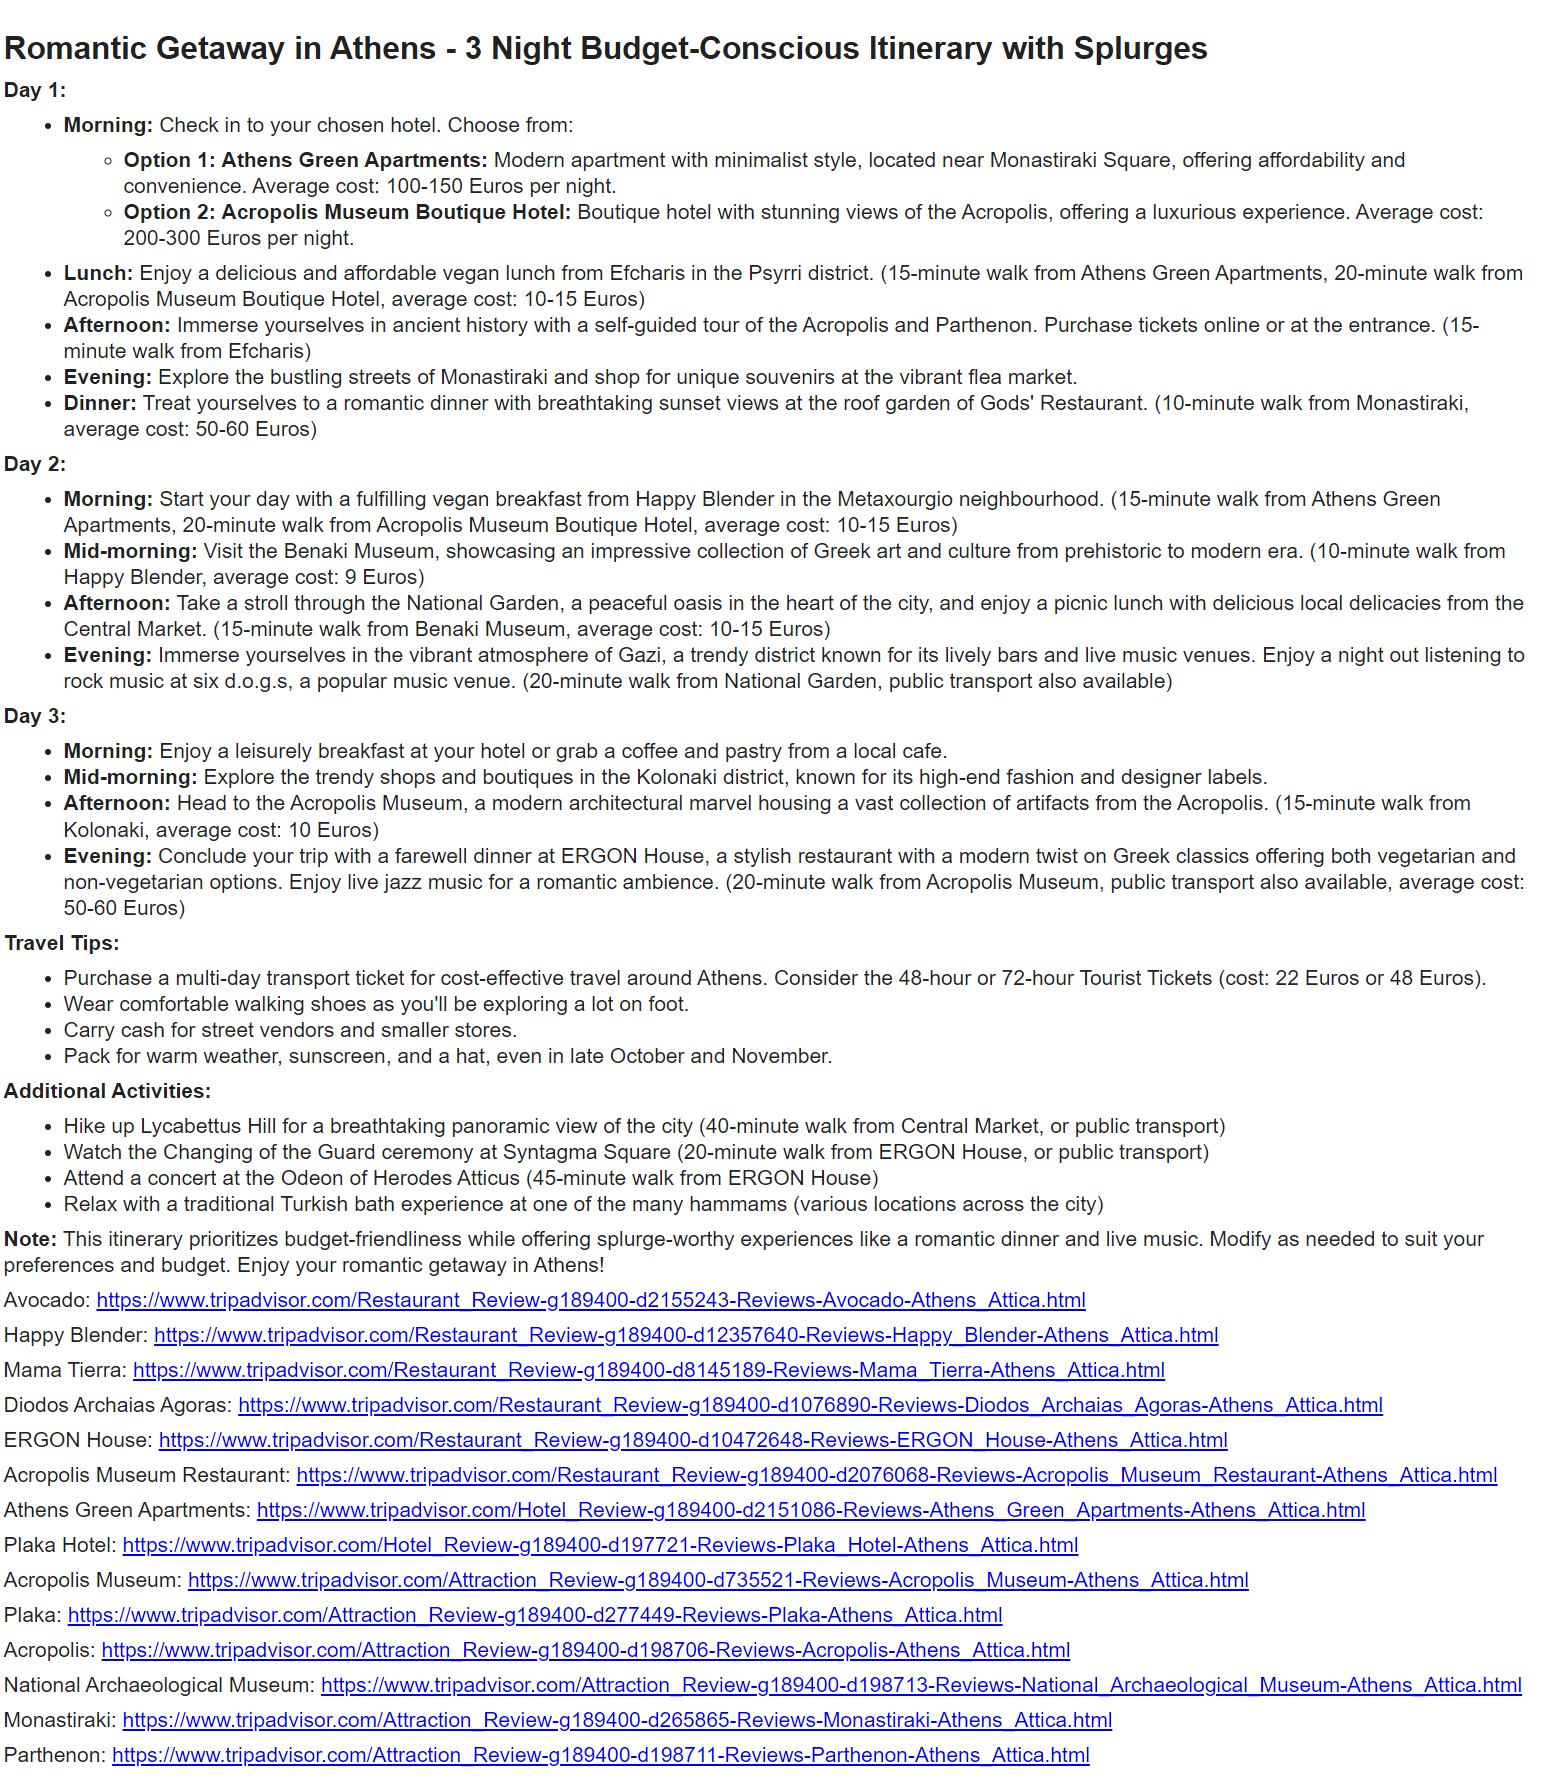
\includegraphics[scale=.8]{finalitinerary}
    \caption{Final Generated Itinerary}
\end{figure}

%%%%%%%%%%%%%%%%%%%%%%%%%%%%%%%%%%%%%%%%%%%%%%%%%%%%%%%%%%%%%%%%%%%%%%%%%%%%%%%%
%%%%%%%%%%%%%%%%%%%%%%%%%%%%%%%%%%%%%%%%%%%%%%%%%%%%%%%%%%%%%%%%%%%%%%%%%%%%%%%%
\chapter{User Survey and Feedback Link}
\begin{enumerate}
\item{\href{https://forms.gle/BpDPoJoUeJ78FSmy7}{User Preference Ingestion Survey Link}}
\item{\href{https://forms.gle/YWLpgBsJyaWhmze57}{User Feedback Survey Link}}
\end{enumerate}


%%%%%%%%%%%%%%%%%%%%%%%%%%%%%%%%%%%%%%%%%%%%%%%%%%%%%%%%%%%%%%%%%%%%%%%%%%%%%%%%
%%%%%%%%%%%%%%%%%%%%%%%%%%%%%%%%%%%%%%%%%%%%%%%%%%%%%%%%%%%%%%%%%%%%%%%%%%%%%%%%

\chapter{Code}

\href{https://gitfront.io/r/am0445/mkaiLCvJ9XdS/Travel-Itinerary-Generation/}{GitHub Repository Link}

\end{document}
